% ====================================================================
% GENERATED FILE -- do not hand-edit.
% Edit bra_rewrite/sections/*.tex, preamble.tex or backmatter.tex,
% then run bra_rewrite/build.sh to regenerate.
% ====================================================================

\PassOptionsToPackage{hyphens}{url}
\PassOptionsToPackage{hidelinks}{hyperref}

\documentclass[preprint,12pt]{elsarticle}

\usepackage[utf8]{inputenc}
\usepackage{amsmath,amssymb,amsfonts}
\usepackage{graphicx}
\usepackage{array}
\usepackage{booktabs}
\usepackage{microtype}
\usepackage{xurl}
\usepackage[section]{placeins}
\usepackage{hyperref}

\graphicspath{{figures/}}

% Prefer slightly looser interword spacing over overfull lines.
\setlength{\emergencystretch}{1.5em}

\journal{Blockchain: Research and Applications}

\begin{document}

\begin{frontmatter}

\title{Fail-Closed Reads, Availability-First Writes: Measured Failure Behavior
of On-Path Ledger Authorization for Legal Document Custody}

\author[uiu]{Golam Bari Fardeen}
\author[uiu]{Namare Shakib Angkon}
\author[uiu]{Syed Zayan Anwar}
\author[uiu]{Md.\ Masum Mizi}
\author[uiu]{Shinthia Rahman}
\author[uiu]{Md.\ Motaharul Islam\corref{cor1}}
\ead{motaharul@cse.uiu.ac.bd}
\cortext[cor1]{Corresponding author.}

\affiliation[uiu]{organization={United International University},
            addressline={United City, Madani Avenue},
            city={Dhaka},
            postcode={1212},
            country={Bangladesh}}

\begin{abstract}
A law firm releases privileged material many times a day, and both the
authorizing table and the release log answer to the firm whose conduct is in
question. Anchoring those records to a blockchain makes tampering evident but
leaves the decision where it was: an immutable log of a wrongful disclosure is
still a wrongful disclosure. Moving the decision onto the ledger closes that gap
in principle; how it behaves when its premises fail remains unreported. We
evaluate a framework in which every download is authorized by a chaincode query
against committed ledger state before any ciphertext or wrapped key is returned.
Documents are browser-encrypted and held in a private InterPlanetary File System
(IPFS) swarm. The design fails asymmetrically, and the asymmetry is this paper's
central result. Reads fail closed: through an induced ledger outage no protected
byte was released, the database never authorized in the ledger's place, and a
grant row forged directly in the database is inert. Writes are availability-first
and can diverge: with ordering unavailable but peers reachable, an access-control
change completes operationally without reaching the ledger. We characterize that
divergence on both mutation paths and show the exposures are mirror images --- a
diverged revocation still serves a revoked user (confidentiality), a diverged
grant still refuses an authorized one (availability) --- and bound both with a
durable outbox that reconverges unattended in a median of 14--16\,s with intent
order preserved. A substituted public key, the design's former sharpest risk, is
now refused at grant time against an immutable ledger-anchored key binding. The
relocated decision costs 4.0 to 4.4\,ms more than a database lookup: a real
difference, not an equivalence, inside a 50\,ms margin fixed in advance. The
ordered heartbeat keeping grant expiry trustworthy costs 7.84\,MB per peer per
day at zero document activity. The asymmetry follows from how reads and writes
reach a ledger, not from this implementation: any design putting enforcement on
the read path inherits it.
\end{abstract}

\begin{keyword}
Blockchain \sep Hyperledger Fabric \sep IPFS \sep
Fail-closed access control \sep Availability under partial failure \sep
Legal document custody
\end{keyword}

\end{frontmatter}

\section{Introduction}
\label{sec:introduction}


\subsection{Administrator-mutable authorization}
\label{sec:problem}

A law firm holding privileged material decides, many times a day, who may read
it. Those decisions are ordinarily enforced by an application server against an
access-control table, and both the table and the record of what was released
are under the control of the organization whose conduct they document. An
administrator, or anyone who obtains their credentials, can widen access, alter
the table, and edit the log that would have shown it.

That arrangement is uncomfortable in ordinary enterprise settings. In
litigation it is untenable. Documents move between firms that are
professionally adverse, to experts and clients, and eventually before a
regulator or a court. Each party must be able to satisfy itself about how the
other handled material it produced, and the party asking is precisely the
party least entitled to be told ``trust our logs.'' Insider action rather than
external intrusion accounts for a substantial share of incidents in the
sector~\cite{ico2024trends,aba2023}, and NIST identifies administrator control
as a first-order risk in permissioned deployments~\cite{nistir8202}.

The difficulty is not that firms keep poor records. It is that the record and
the decision have the same custodian. Verification therefore terminates at the
organization being verified.

\subsection{Limitations of record anchoring}
\label{sec:anchoring_insufficient}

The established response is to anchor: hash each document and each significant
event, commit the hashes to a ledger the consortium shares, and let any member
verify later that a record has not been altered. This works, and it is what
most blockchain-based evidence and document systems do.

It also leaves the decision where it was. Anchoring establishes that a release
was recorded; it does not establish that the release was authorized. An
immutable log of a wrongful disclosure is still a wrongful disclosure, and the
log is only as complete as the application chose to make it: an application that never records a refused attempt leaves a probing adversary invisible, and
one that has already released the document cannot un-release it by writing a
row. Tamper-evidence after the fact and enforcement at the moment of release
are different properties, and only the second constrains what an administrator
can actually do.

Moving the decision itself onto the ledger closes that gap in principle: the
release path consults committed, consortium-visible state before returning
anything, so an administrator who edits the operational database changes
nothing that matters. The principle is not new. What is unexamined is what the
move \emph{costs} and, more importantly, how it behaves when its own premises fail: when the ledger is unreachable, when the adversary holds the database
it was meant to displace, or when the mechanisms that make the decision
trustworthy turn out to carry standing costs of their own. Those failure modes
are not incidental to the design; they are where its guarantees are actually
decided. This paper measures them.

\subsection{Research questions}
\label{sec:rqs}

\begin{description}

\item[RQ1: Relocation and its verification.] Can the document-release
decision be evaluated against committed ledger state rather than against
state the application controls, and does that relocation survive an adversary who
holds write access to the operational database? The second half is the part
usually asserted rather than tested, and it is what distinguishes a relocated
enforcement boundary from a decorated one.

\item[RQ2: Cost, in latency and in capacity.] What does the relocated
decision cost on the interactive path, and what capacity does the resulting
system sustain? We fix the read-path threshold in advance at 50\,ms, a
deliberately conservative half of the 100\,ms below which feedback is perceived
as instantaneous~\cite{nielsen1993usability}, and the write threshold at
5\,s, within the ten-second limit beyond which a background task loses the
user's attention~\cite{miller1968response,nielsen1993usability}. Capacity is assessed against a synthetic steady state and its
burst multiple, both stated as assumptions rather than as measurements of real
legal traffic.

\item[RQ3: Behavior under unavailability.] What does the design do when
the ledger, or part of it, cannot be reached? This question is asked separately
of reads and of writes, because they reach the ledger by different routes and,
as it turns out, fail differently.

\item[RQ4: Scale.] How does cost grow with the archive, with the size of the
consortium, and with elapsed time? The third axis is included because the
mechanism that makes grant expiry trustworthy accrues cost whether or not the
system is used at all.

\end{description}

RQ1 is answered in Sections~\ref{sec:exp_latency},
\ref{sec:exp_db_mutation} and~\ref{sec:exp_pubkey}, RQ2 in
Sections~\ref{sec:exp_latency}, \ref{sec:exp_throughput}
and~\ref{sec:exp_durable_baseline}, RQ3 in Sections~\ref{sec:exp_failclosed},
\ref{sec:exp_divergence} and~\ref{sec:exp_timeanchor}, and RQ4 in
Sections~\ref{sec:exp_ledgergrowth} and~\ref{sec:exp_netscale}.


\subsection{Contributions}
\label{sec:contributions}

Placing an authorization decision on a content-retrieval path is not by itself
new. Steichen et al.~\cite{steichen2018blockchain} gated IPFS retrieval on a
smart contract, and the recent RBAC-IPFS scheme of Liu et
al.~\cite{liu2026rbacipfs} both performs and measures such a check. What has not
been reported is how an on-path enforcement design \emph{behaves when its
premises fail}: when the ledger is unreachable, when an adversary holds the
database the ledger was meant to displace, and when the mechanisms that make the
decision trustworthy are themselves priced. Each contribution below is a
measurement of that kind.

\begin{enumerate}

\item \textbf{Measured asymmetric failure behavior across the read and write
paths, and a taxonomy that explains it.} Reads fail closed: through an induced
ledger outage the release path released no protected byte and never fell back to
the operational access-control list (Section~\ref{sec:exp_failclosed}). Writes
are availability-first and can diverge, and we characterize the divergence on
both access-control mutation paths rather than one. With the ordering service
unavailable but peers reachable, an access-control change completes operationally
without reaching the ledger; a diverged revocation then still serves a revoked
user and a diverged grant still refuses an authorized one
(Section~\ref{sec:exp_divergence}). These are mirror-image exposures ---
confidentiality and availability --- and the direction is set by the fail-closed
read, not by the implementation, which is the taxonomy we report. A durable
outbox bounds both, reconverging unattended in a median of 14--16\,s with intent
order preserved across mixed grant/revoke queues. No system in our comparison
reports measured behavior under ledger unavailability at all, in either
direction.

\item \textbf{A relocation of release-path authorization verified adversarially
on both the forged-row and the substituted-key attack.} That the ledger
\emph{decides} is easy to assert and rarely tested. We test it by performing the
mutations an attacker with write access to the operational store would perform: a
forged grant row yields nothing, because the chaincode and not the database
authorizes (Section~\ref{sec:exp_db_mutation}); and a substituted public key is
refused at grant time against an immutable ledger-anchored key binding
(Section~\ref{sec:exp_pubkey}), closing what the prior version identified as its
sharpest residual risk. The same experiments bound the claim: deleting a
legitimate row does not revoke, so a database edit must not be read as a
revocation, and an unbound legacy user is still grantable under a stated
migration posture. The decision costs 4.0 to 4.4\,ms above an equivalent database
lookup (Section~\ref{sec:exp_latency}), consistent in magnitude with the on-path
costs reported for generic file sharing~\cite{liu2026rbacipfs}; the contribution
is the adversarial verification rather than the figure.

\item \textbf{The standing price of clock trust, and a scale characterization
that had to be corrected because of it.} Grant expiry is evaluated against a
timestamp the calling gateway supplies, so an ordered heartbeat is required to
make it trustworthy. That heartbeat is not free in a way that is easy to miss:
it accrues 7.84\,MB per day per peer with no document activity whatsoever, and
over a ten-year retention horizon it exceeds the cost of a million stored
documents several times over (Section~\ref{sec:exp_ledgergrowth}). A security
mechanism whose price is permanent, activity-independent storage is a design
consideration we have not seen reported. It also invalidated our own earlier
model of the system: storage is linear in documents \emph{and} in time, not in
documents alone. The document and topology axes are characterized alongside it: query cost flat across three orders of
magnitude of world state, throughput declining 5.5\,\% from two to seven
organizations (Section~\ref{sec:exp_netscale}); and the trade-off against the heartbeat
interval is measured in both directions (Section~\ref{sec:exp_timeanchor}).

\item \textbf{An end-to-end price against a baseline that keeps its own
promise.} The architecture this work displaces treats the ledger as a passive
audit log, and pricing against a careless implementation of it would prove
nothing. Rebuilt so that its audit trail actually survives a restart, that
baseline sustains under a third of the throughput of on-path enforcement at
both of the two concurrency levels measured
(Section~\ref{sec:exp_durable_baseline}, whose sweep is reduced and does not
re-validate saturation). The reason is structural. In the
audit-log architecture the anchor \emph{is} the enforcement record, so it must
be durable and must keep pace with the request rate; on the release path the
decision precedes release, so the anchor is telemetry and need be neither. To
our knowledge no prior system prices on-path enforcement against the
architecture it replaces.

\end{enumerate}

\paragraph{What is deliberately not claimed}
No new access-control primitive is proposed, and the cryptographic construction
composes standard parts in a standard arrangement rather than contributing one;
Section~\ref{sec:security_properties} states which security properties follow
from it and which do not.


\subsection{Paper organization}
\label{sec:organization}

Section~\ref{sec:related} places the work against the closest systems and
defines the comparison this paper's novelty claim rests on.
Section~\ref{sec:threat_model} fixes the assumptions, adversaries, and claimed
properties, and states the boundary between the framework and the prototype
that was measured; read it early, because several later claims hold of one and
not the other. Sections~\ref{sec:architecture}, \ref{sec:crypto}
and~\ref{sec:implementation} describe the system: where the authorization
decision sits, what protects document content, and what was actually built.

Section~\ref{sec:performance} is the evaluation. It opens by fixing the testbed
and the statistical conventions that govern every number in it, then prices the
relocated decision, tests whether it holds against an adversary and under
outage, measures what it costs to keep running, and finally prices the whole
architecture against the one it replaces.

Section~\ref{sec:discussion} draws out what the measurements do and do not
establish, and Section~\ref{sec:conclusion} closes.

One convention is worth stating in advance. Limitations are reported where the
result they qualify is reported, rather than gathered into a section at the
end. A reader who stops after any single measurement should already know what
that measurement does not show.


\section{Background and related work}
\label{sec:related}

\subsection{Hyperledger Fabric}
\label{sec:fabric}

Fabric is a permissioned ledger in which participants hold X.509 identities
issued under organizational membership providers~\cite{androulaki2018hyperledger}.
Two distinctions matter throughout this paper. A \emph{query} is answered
locally by a single peer against its committed world state; a \emph{submit} is
endorsed, ordered into a block, and validated before it changes that state.
Read-side authorization is therefore cheap and locally answerable, while any
state change must pass the ordering service. Almost every asymmetry we report
follows from that split.

The world state is a key-value store, so an access decision expressed as a
lookup by document identifier costs one read regardless of archive size, a property
Section~\ref{sec:exp_ledgergrowth} confirms across three orders of
magnitude. Channels and private data collections partition data between subsets
of members, but both are \emph{network-level}: they determine who can see a
channel, not whether a particular request for a particular document is
authorized.

\subsection{Content-addressed off-chain storage}
\label{sec:ipfs}

IPFS addresses content by hash~\cite{benet2014ipfs}: a stored object's
identifier is derived from its bytes, so substituting content changes its
address and is detectable. Files above a threshold are split into blocks
arranged as a Merkle directed acyclic graph, and peers exchange those blocks
concurrently. Content addressing gives integrity, not confidentiality and not access control (any peer holding an identifier can request the
object), which is precisely the gap the systems reviewed below try to close.

\subsection{Related systems}
\label{sec:related_systems}

\subsubsection{Anchoring and integrity-only systems}
An established line of work uses a ledger to make records tamper-evident.
Judicial evidence preservation~\cite{liu2024blockchain}, two-level evidence
chains~\cite{twoLevelBlockchain}, timestamped judicial
records~\cite{verma2021nyaya}, chain-of-custody
auditing~\cite{hanafi2021ipfschain}, and applied instruments such as digital
wills~\cite{hernando2025wills} all establish that a record existed and has not
been altered. None places a decision on the retrieval path: the ledger records
what the application did, and the application decides. This is the architecture
Section~\ref{sec:exp_durable_baseline} prices against.

\subsubsection{Hybrid storage without an on-path decision}
A second line pairs anchoring with off-chain storage for
scale~\cite{liu2024blockchain,jlil2024blockchain}, and NFT-based evidence
registration extends it with fog computing~\cite{peelam2026decentralized}. The
pattern is sound and orthogonal to ours (we use it too), but a hash proves
a retrieved payload matches a prior record; it does not enforce who may
retrieve it.

\subsubsection{Multi-party and Fabric-based evidence systems}
Closer to the legal-consortium setting, Onyeashie et
al.~\cite{onyeashie2025fabricEvidence} separate law-enforcement, forensic and
judicial workflows across three Fabric channels, with role privileges enforced
at the API and zero-knowledge proofs used for evidence \emph{integrity}. Guo et
al.~\cite{guo2024efficient} combine Fabric and IPFS for medical records,
verifying user identity in chaincode with zero-knowledge proofs at registration
and governing subsequent sharing through proxy re-encryption. Both are
substantial systems, and both illustrate why our comparison column has to be
defined carefully: channel membership and identity verification are real
access-control mechanisms, but neither evaluates a per-document decision at the
moment of retrieval.

\subsubsection{Access-control-centric systems}
\label{sec:acl_systems}
A fourth line makes the access decision the contribution, and it is where our
closest neighbors sit.

Steichen et al.~\cite{steichen2018blockchain} are the architectural ancestor.
Their \texttt{acl-IPFS} modifies the storage daemon so that a
\texttt{checkAccess} contract call gates retrieval per chunk, with an Ethereum
contract holding the list: once a file is added, no one but the owner can
retrieve it until access is granted. That is a genuine on-path authorization
decision, and we claim no priority over it.

Liu et al.~\cite{liu2026rbacipfs} bring the idea to a consortium ledger and
solve its central inefficiency. Their RBAC-IPFS hooks the block-exchange
decision engine so that permissions are checked before a block is served, but
authorizes only the \emph{root} identifier on-chain and lets every sub-block
inherit that decision through a locally verified Merkle path: constant on-chain cost per download rather than one call per block, with completeness,
soundness and no-bypass proved formally. They report contract execution in
1--2\,ms and end-to-end retrieval in 146--156\,ms under an emulated wide-area
network, together with an adversarial evaluation covering sub-block injection
and denial of service.

RBAC-IPFS is both the nearest system and a stronger result than ours in two
respects: it has formal
proofs, which we do not, and its root-anchoring makes on-chain cost independent
of file size, which ours is not. Three things differ. First, enforcement sits
at a different layer: RBAC-IPFS gates \emph{block routing} at the storage
plane, whereas the decision we measure gates an application release path that
also hands out per-recipient key material, and their own paper identifies
payload confidentiality as an open limitation, proposing short-lived keys, key
rotation or proxy re-encryption as future mitigations. Second, time-bounded
access appears in that same list of future work; grant expiry, and the clock
trust it depends on, is measured here rather than proposed
(Section~\ref{sec:exp_timeanchor}). Third, and most consequentially for this
paper, RBAC-IPFS does not examine what happens when the ledger it depends on
becomes unreachable. Its adversarial evaluation concerns the storage layer.

Three systems bound the space. FileWallet~\cite{chen2022filewallet} validates
chaincode privilege checks functionally without timing them; Mukta et
al.~\cite{mukta2026zerotrust} benchmark zero-trust capability verification on
Fabric, but the capability is checked \emph{before} retrieval rather than on it:
their storage tier is issuer-hosted cloud storage that never consults the
ledger, so no release is gated by the verified capability; and Notash et al.~\cite{notash2026adaptive} analyze adaptive
e-health policies formally while reporting workflow-scale averages rather than
isolating the enforcement decision. Generic capability and attribute
systems~\cite{macaroons2014,zanzibar2019,hu2014guide} are more expressive than
anything here, but their enforcement authority is a service layer rather than
consortium-visible state, a difference in trust model rather than in policy
power.

\subsection{Comparison}
\label{sec:comparison}

Table~\ref{tab:related} compares the systems on four properties. The first
requires definition, because it is the one most easily overstated.

\textbf{Release-path authorization} means an authorization decision evaluated
against ledger state, \emph{per protected object}, on the request that returns
it, before content or key material is released. Network-level partitioning
scores \textbf{P}, not \textbf{Y}: channel membership determines which
organizations can see a data set, and it is a real control, but it does not
decide an individual request. Identity verification performed once at
enrollment likewise scores \textbf{P}. A system scores \textbf{Y} only if a
per-object check stands between the request and the bytes.

\begin{table}[!t]
\centering
\caption{Comparison with the closest systems. Rel: release-path authorization
as defined in Section~\ref{sec:comparison}. Key: per-recipient distribution of
document key material. Exp: time-bounded grants enforced by the ledger. Out:
\emph{measured} behavior when the ledger is unavailable. Y supported,
P partial, N not supported.}
\label{tab:related}
\footnotesize
\setlength{\tabcolsep}{4pt}
\begin{tabular}{@{}>{\raggedright\arraybackslash}p{0.30\columnwidth}%
                 >{\raggedright\arraybackslash}p{0.24\columnwidth}cccc@{}}
\toprule
System & Platform & Rel & Key & Exp & Out \\
\midrule
Steichen et al.~\cite{steichen2018blockchain} & Ethereum + modified IPFS
  & Y & N & N & N \\
Liu et al.\ (RBAC-IPFS)~\cite{liu2026rbacipfs} & Fabric + modified IPFS
  & Y & N & N & N \\
Chen et al.~\cite{chen2022filewallet} & Fabric + IPFS & P & N & N & N \\
Guo et al.~\cite{guo2024efficient} & Fabric + IPFS & P & Y & N & N \\
Onyeashie et al.~\cite{onyeashie2025fabricEvidence} & Fabric + IPFS
  & P & N & N & N \\
Notash et al.~\cite{notash2026adaptive} & Fabric + IPFS & P & N & P & N \\
Mukta et al.~\cite{mukta2026zerotrust} & Fabric + SSI & N & N & Y & N \\
Anchoring systems~\cite{liu2024blockchain,twoLevelBlockchain,verma2021nyaya,hanafi2021ipfschain,peelam2026decentralized}
  & various + IPFS & N & N & N & N \\
\midrule
This work & Fabric + IPFS & Y\,(reads) & Y & Y & \textbf{Y} \\
\bottomrule
\end{tabular}
\end{table}

Two columns carry the argument. \textbf{Key} separates systems that decide
\emph{whether} a request is authorized from systems that also control
\emph{what material} the requester can decrypt; only Guo et al., through proxy
re-encryption, and this work distribute per-recipient key material. \textbf{Out}
is empty for every prior system. None reports what its enforcement point does
when the ledger backing it cannot be reached; that is not a criticism of those systems, whose
contributions lie elsewhere, but an observation about what
the literature has and has not measured.

Our own \textbf{Y} in the first column is qualified in the table itself,
because it holds for reads and not for writes
(Section~\ref{sec:exp_divergence}), and the qualification is carried in the
table rather than a footnote because the asymmetry is a result of this paper.

\subsection{Research gaps}
\label{sec:gaps}

Three gaps follow. \textbf{On-path enforcement is unmeasured under
failure:} placing a decision on the retrieval path is established
practice~\cite{steichen2018blockchain,liu2026rbacipfs}, but a design that fails
closed and one that silently falls back are indistinguishable in every paper
reviewed above. \textbf{The relocation is asserted rather than adversarially
tested:} we have found no system that performs the mutation an attacker with
database access would perform and reports what the release path then does. And
\textbf{the mechanisms that make a decision trustworthy are not priced:}
time-bounded access appears as future work in the closest
system~\cite{liu2026rbacipfs}, and where expiry does exist it is generally
enforced cryptographically, by issuing time-limited key material and refreshing
ciphertext on a cycle~\cite{cai2023timebound}. That sidesteps rather than
answers the question a runtime decision faces: which clock the expiry is
evaluated against, and who supplies it.


\section{Threat model, assumptions, and scope}
\label{sec:threat_model}

A narrow claim is only credible if the conditions under which it holds are
stated first. The deployment model throughout is a permissioned consortium of
known and legally accountable institutions (law firms and a regulator, each
authenticated through Fabric membership services) in which state-changing
transactions are validated against an endorsement policy before being ordered
and committed.

\subsection{Assumptions}
\label{sec:assumptions}

\begin{description}
\item[A1 Cryptographic primitives and transport.] The adversary is a Dolev-Yao
attacker~\cite{dolev1983security} on the network: it may be adaptive, but cannot
break AES-256-GCM, ECDSA or ECDH over P-256, or SHA-256. Peers and the ordering
service present TLS certificates that the gateway validates against the
consortium TLS certificate authority~\cite{rescorla2018tls}, so integrity and
authenticity of the gateway-to-peer channel are assumed rather than derived: a
decision returned by a peer reaches the gateway unmodified. Availability of that
channel is \emph{not} assumed, and is the subject of RQ3.

\item[A2 Ordering bound.] Of three ordering nodes at most one crash-fails, and
no orderer behaves Byzantinely. This bounds block formation only.

\item[A3 Endorsement quorum.] No coalition sufficient to satisfy the channel
endorsement policy colludes. Committing peers independently validate
endorsement signatures and read-write sets, so a single organization cannot
fabricate valid state. A2 and A3 are independent bounds.

\item[A4 Storage availability.] At least one honest storage node holding a
document's ciphertext remains reachable. Integrity does \emph{not} rest on
this, because hash anchoring detects tampering under A1; only availability
does.

\item[A5 Identity table.] The table binding users to their public keys has not
been maliciously modified. This is deliberately the weakest assumption in the
prototype; its violation is Scenario~S3 (Section~\ref{sc:s3}), and discharging it requires
ledger-anchored key registration, which is not implemented.

\item[A6 Client endpoint.] The user's browser is uncompromised while keys are
unlocked and plaintext is present.

\item[A7 Gateway clocks.] Grant expiry is evaluated against a timestamp that,
on a query rather than an ordered transaction, originates in the caller's
proposal, and under custodial submission the caller is the application
gateway. The ordered time anchor constrains this rather than removing it:
backdating is bounded by how stale the anchor is permitted to become, and what
remains assumed is that the anchor is refreshed
(Section~\ref{sec:exp_timeanchor}). This is the assumption most specific to
custodial deployment, and per-user enrollment does not discharge it, because a
query is never ordered and so carries no ordering-service timestamp to
substitute.
\end{description}

\subsection{Adversary classes}
\label{sec:adversaries}

\begin{table}[!t]
\centering
\caption{Adversaries in scope, what each is prevented from achieving, and by
what; residuals are expanded in Sections~\ref{sec:scenarios}
and~\ref{sec:scope}.}
\label{tab:adversaries}
\footnotesize
\setlength{\tabcolsep}{4pt}
\begin{tabular}{@{}>{\raggedright\arraybackslash}p{0.20\columnwidth}%
                 >{\raggedright\arraybackslash}p{0.36\columnwidth}%
                 >{\raggedright\arraybackslash}p{0.36\columnwidth}@{}}
\toprule
Adversary & Prevented from & Residual \\
\midrule
Honest-but-curious peer &
Reading document content; all payloads are ciphertext held off-chain &
Sees content identifiers, timestamps, and the access graph; can confirm a
candidate document from its anchored hash \\
Database administrator &
Authorizing a release; the ledger decides, measured in
Section~\ref{sec:exp_db_mutation} &
Cannot revoke by deletion either, which is easy to misread as revocation \\
Compromised gateway &
Forging ledger state. Rewinding the committed time anchor rests on multi-peer
endorsement and is argued rather than tested
(Section~\ref{sec:exp_timeanchor}) &
Supplies the query timestamp (A7); can substitute a recipient key before a
grant is formed \\
Compromised browser &
Nothing, once keys are unlocked &
Out of scope under A6 \\
Compromised storage node &
Substituting content undetectably; the anchored hash fails to match &
Degrades to loss of availability (A4) \\
Two colluding orderers &
Committing invalid state; peers revalidate independently &
Can censor or delay, which crash-fault tolerance does not prevent \\
\bottomrule
\end{tabular}
\end{table}

Two of the classes in Table~\ref{tab:adversaries} are worth separating from the
rest. The \emph{database administrator} is the adversary the architecture exists
to defeat, and the one whose defeat this paper measures rather than argues. The
\emph{compromised gateway} is the adversary it defeats least well, because
custodial submission leaves it holding both the submitting identity and the
clock.

\subsection{Security properties}
\label{sec:security_properties}

Four properties are claimed, each argued under the assumptions above and pointed
at the evidence supporting it. Machine-checked verification is future work, but
the property set is fixed here so that such work has a target.

\begin{description}
\item[P1 Ledger-gated release.] Under A1--A3 and A5--A7, neither ciphertext nor
a wrapped document key is returned on the evaluated download path unless a
chaincode evaluation against committed ledger state authorizes the requester at
request time. \emph{Evidence:} Section~\ref{sec:exp_db_mutation}, where a grant
forged directly in the operational store yields no release. Two qualifications
bound it. Grant \emph{membership} is ledger-evaluated in the full sense; grant
\emph{expiry} is ledger-evaluated only up to the clock the caller supplies, so
P1's expiry component is weaker than its membership component and is bounded by
A7. And the prototype evaluates against a single peer, so P1 additionally
assumes that peer returns honest world state.

\item[P2 Fail-closed reads.] Under A1, if the ledger cannot be consulted the
download path denies rather than falling back to operational state.
\emph{Evidence:} Section~\ref{sec:exp_failclosed}: no protected byte released
across an induced outage, no fallback authorization, and denials recorded with
their cause. This is a read-path property. Writes are availability-first by
design and can diverge from the ledger during an ordering outage; that divergence
is characterized on both access-control paths and bounded by a durable outbox
(Section~\ref{sec:exp_divergence}).

\item[P3 Tamper evidence.] Under A1, any change to the stored ciphertext is
detected before use: the hash anchored at registration cannot be matched by
altered content without breaking SHA-256. Availability, by contrast, depends on
A4.

\item[P4 Attributable ledger actions.] Under A1--A3, every grant, revocation and
anchored audit event is attributable to the submitting organization through
membership signatures, and document commitments are additionally bound to
user-level signing keys, subject to the custodial-identity limit of
Section~\ref{sec:scope} and to A5.
\end{description}

\subsection{Attack scenarios}
\label{sec:scenarios}

\subsubsection{S1 Revoked-credential replay}
A formerly authorized user requests a document after revocation. The application
cannot serve from cached state, because P1 places the evaluation on the request
itself, and the denial is anchored to the ledger like a grant, so a refused
attempt is independently verifiable rather than resting on the honesty of the
server that refused it (Section~\ref{sec:exp_db_mutation}). This holds
\emph{provided the revocation has committed}: one issued while ordering is
unavailable updates the operational store but not the ledger, and the release
path keeps authorizing from the stale grant until re-anchoring completes
(Section~\ref{sec:exp_divergence}).

\subsubsection{S2 Induced-outage fallback}
An insider disrupts the ledger deliberately, expecting the application to fall
back to a table they can edit. Under P2 it does not
(Section~\ref{sec:exp_failclosed}), and the storage-tier analogue behaves the
same way: disabling replicas degrades availability but never substitutes
content.

\subsubsection{S3 Public-key substitution}
\label{sc:s3}
In the prior version of this system this was the sharpest residual risk. An
adversary violating A5 replaces a user's public key before a grant is formed;
subsequent grants would wrap the document key under the attacker's key while the
ledger commits a cryptographically valid transaction whose recipient binding is
semantically wrong, so P1 held mechanically while its authorization was subverted
upstream. The wrapped-key token binds the recipient's identity as associated
data, but that does \emph{not} help here: an adversary who substituted the public
key holds the matching private key and supplies the legitimate identifier
unchanged.

This is now closed by a ledger-witnessed user-to-key binding, and the closure is
measured rather than argued (Section~\ref{sec:exp_pubkey}). Enrollment anchors a
hash of the user's wrapping key on the ledger, immutably; the grant path requires
the granter to attest the key it wrapped under, and the chaincode refuses the
grant when the attestation does not match the anchor. A key substituted in the
operational table then fails at grant time, in consortium-visible state, exactly
as a forged access-control row fails on the read path. The residual is a
migration one: while any user enrolled before anchoring remains unbound, the
grant to that user proceeds and is audited as such, and closing this fully
requires back-anchoring outstanding users' keys.

\subsubsection{S4 Storage-tier substitution}
A compromised storage node serves modified ciphertext for a known identifier. P3
backstops this end to end: the client verifies decrypted plaintext against
the anchored hash before accepting the document, so under A1 the attack degrades
into denial of availability regardless of how many nodes collude.

\subsubsection{S5 Gateway-side backdating}
A compromised gateway holds a document whose grant has expired and constructs a
query carrying a timestamp from before the expiry instant. Nothing in the ledger is
falsified (the adversary supplies the clock, not the policy), so signature checking and endorsement do not detect it. The time anchor bounds the
reachable window rather than closing it, as set out under A7 and measured in
Section~\ref{sec:exp_timeanchor}. Two limits matter: the gateway is also what
submits heartbeats, so it can starve the anchor even though it cannot rewind it;
and no backdated proposal was constructed against the deployment, so the defense
is measured for enforcement cost while the attack itself is analyzed rather than
demonstrated.

\subsection{Scope: framework, prototype, and what is out of scope}
\label{sec:scope}

Throughout this paper we distinguish the \emph{framework}, the intended
security architecture, from the \emph{prototype}, which is what was measured.
The distinction is load-bearing, because several claims hold of one and not the
other, and three gaps matter most. \textbf{Fabric identities are custodial:} the
gateway submits with organization-level credentials rather than per-user
certificates, so ledger transactions are attributable to an organization and not
to a person, and A7 is a direct consequence. \textbf{Private keys live in
browser storage} under a password-derived wrapping key, which resists passive
theft but not an active endpoint compromise. \textbf{Key wrapping binds
recipient identity but not document identity,} so a token cannot be re-targeted
to a different principal but can in principle be replayed across documents for
the same one; and tokens minted before the binding was introduced are still
accepted, leaving the guarantee advisory until outstanding grants are reissued.

Out of scope, each with the assumption it would violate: Byzantine ordering
behavior (A2); collusion of an endorsement quorum (A3); endpoint compromise
(A6); traffic analysis of on-chain metadata, which remains visible to channel
members and is discussed as a design tension rather than solved; network-layer
denial of service beyond the measured outage scenarios; and side-channel attacks
on the cryptographic implementations.

Byzantine ordering deserves one sentence more, because it is a choice and not an
oversight. The prototype uses a crash-fault-tolerant ordering service, which
tolerates node failure but not malicious ordering. Legal accountability among
distinct institutions lowers the probability of collusion; it supplies no
cryptographic bound. Deployments needing one should use a
Byzantine-fault-tolerant ordering
service~\cite{castro1999pbft,stathakopoulou2022smartbft},
supported in Fabric as a channel-level
configuration~\cite{fabricBFTConfigurationDoc}: a migration that changes
ordering and channel configuration but not the document-management chaincode.


\section{System architecture}
\label{sec:architecture}

\subsection{Overview and topology}
\label{sec:topology}

The deployment (Fig.~\ref{fig:topology}) is a three-organization consortium: two law firms and a
regulator, each running a peer with its own CouchDB state
database~\cite{fabricCouchDBStateDB_v24} on a shared
channel~\cite{fabricChannelsDoc},
with a three-node Raft ordering
service~\cite{Ongaro2014,hyperledgerFabricOrderingService_v24} distributed
across the members, so no single institution controls transaction ordering. Encrypted payloads live in a
private content-addressed swarm; the ledger holds document metadata, hashes,
content identifiers, and the access-control state that decisions are evaluated
against. Between the client and both tiers sits an application gateway, which
terminates authentication, submits and queries the ledger, and retrieves
ciphertext: all three paths in Fig.~\ref{fig:topology} (ordered
submission, local evaluation, and ciphertext retrieval) pass through it.
The gateway is deliberately \emph{not} trusted for authorization
decisions (that is the point of the architecture), but it remains trusted
for identity submission, because it submits with custodial Fabric
credentials. That is where A7 comes from
(Section~\ref{sec:assumptions}).

\begin{figure}[!t]
    \centering
    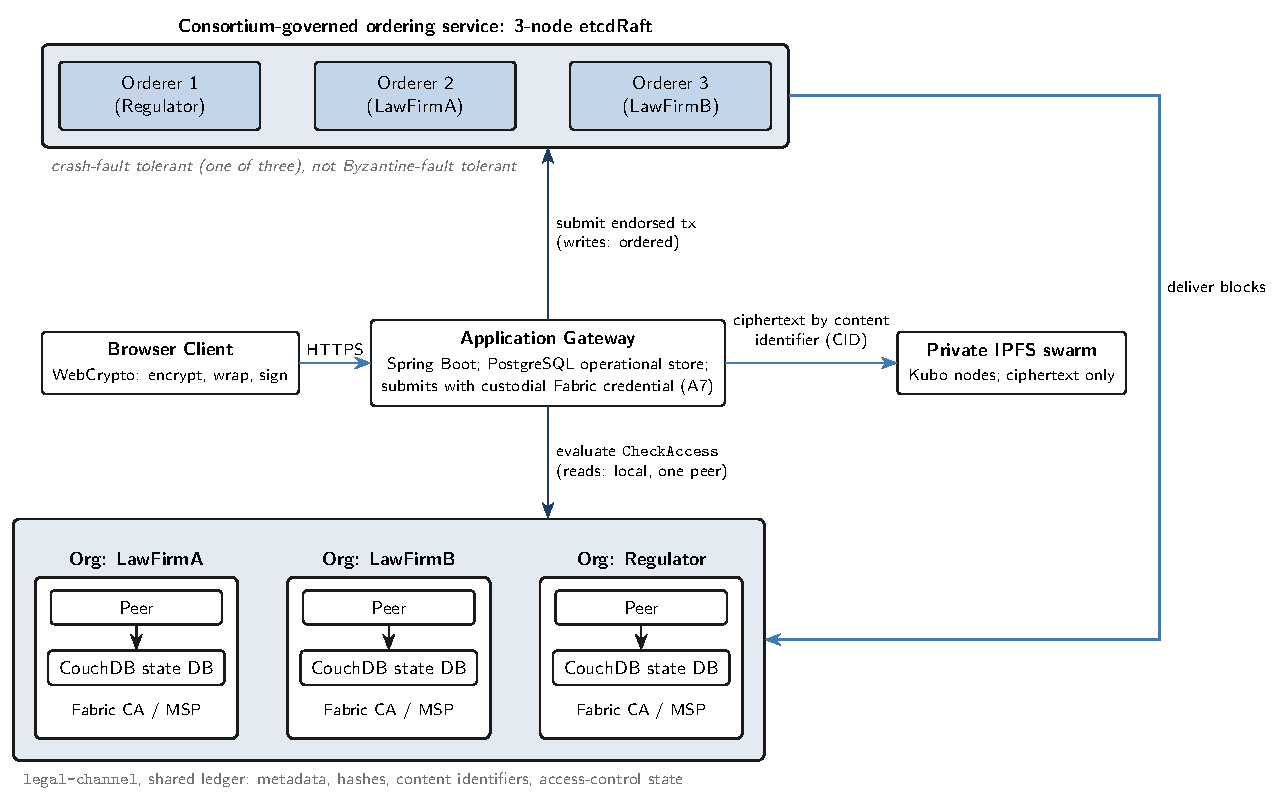
\includegraphics[width=\columnwidth]{fabric_topology6.pdf}
    \caption{Topology of the evaluated deployment: three peer organizations
    on a shared channel, a three-node ordering service distributed across
    the members, and a private storage swarm holding ciphertext only.}
    \label{fig:topology}
\end{figure}

\subsection{Roles and identity}
\label{sec:roles}

Within a firm, roles run from partners with full matter visibility down to
paralegals restricted to assigned documents (Fig.~\ref{fig:hierarchy}). The
distinction that several of this paper's claims turn on is where each is
enforced: intra-organization role structure at the application layer, from the
authenticated session; cross-organization access by the ledger. The prototype
submits ledger transactions with organizational credentials rather than per-user
certificates issued under the organizational membership service
provider~\cite{fabricMSP}, so a ledger transaction is attributable to a firm and
not to a person. User-level signatures bind a signing key to specific document content,
which is a different and weaker property than per-user ledger attribution.

\begin{figure}[!t]
    \centering
    
\includegraphics[width=\columnwidth]{Hierarchy.pdf}
    \caption{Role hierarchy within a firm; roles are enforced at the
    application layer, release of protected material by the ledger
    (Section~\ref{sec:twolayer}).}
    \label{fig:hierarchy}
\end{figure}

\subsection{Two-layer authorization}
\label{sec:twolayer}

Two independent layers must both permit a request before protected material is
returned. \textbf{Layer 1} is role-based authorization at the gateway, evaluated
from the authenticated session before any business logic runs; it is ordinary
application security and carries none of this paper's claims. \textbf{Layer 2}
is the chaincode decision, which reads the document's access-control map from
committed ledger state and evaluates two branches in order: an entry keyed by
the requesting user, then one keyed by the requesting organization. Each may
carry an expiry, checked against the transaction timestamp. If neither branch
authorizes, the decision is negative. State-changing calls are additionally
subject to the channel endorsement policy~\cite{fabricEndorsementDoc}; the
release-path decision is an evaluate and is not.

There is no third branch. An implicit ownership fallback (authorizing any
member of the owning organization for any of that organization's documents,
given only a document identifier) was removed after
Section~\ref{sec:exp_db_mutation} measured it end to end. In legal practice
that over-permission is not minor, since ethical walls and matter-level
screening are the primary intra-firm access requirement. Every principal
requires an explicit grant; document registration issues one to the uploader, so
upload-then-download works without a special case.

\subsection{The release path}
\label{sec:releasepath}

Two endpoints return protected material, one serving ciphertext and the
other the recipient's wrapped document key, and both pass the same fail-closed gate,
which resolves in one of four ways. A requester with no organizational binding
is refused before the ledger is consulted at all. If the ledger cannot be
reached, the request is refused with a service-unavailable status and an outage
denial is recorded, with no fallback to the operational access-control list,
which is the property Section~\ref{sec:exp_failclosed} measures. If the
chaincode returns a negative decision, the request is refused and the denial is
anchored to the ledger alongside grants, so a refused attempt is independently
verifiable rather than resting on the honesty of the server that refused it.
Only a positive decision releases anything.

The two endpoints then diverge. Ciphertext is
fetched from storage by content identifier; the wrapped key is served from the
requester's own operational access entry. So the ledger decides \emph{whether}
to release, while the operational store determines \emph{which} key material
exists to release. Section~\ref{sec:exp_db_mutation} measures both directions of
that split, including the consequence that deleting an operational row does not
revoke ledger-authorized ciphertext access.

\paragraph{Scope of the ledger decision}
Collaborative features built around a document (annotation, and the
subscription authorization behind it) use an operational access check rather
than a ledger round trip, because a chaincode call per annotation event would be
disproportionate. This is a deliberate scope boundary: release of protected
material is ledger-gated; ancillary collaboration around an already-released
document is not.

\subsection{Grant, expiry, and revocation}
\label{sec:grants}

A grant is a ledger entry naming a principal, an operation, and an optional
expiry instant. Issuing one also wraps the document key under the recipient's
public key, so authorization and key distribution are established together
rather than the first implying the second.

Expiry is evaluated inside the access decision against the transaction
timestamp, which is deterministic across endorsing peers; this is necessary, since a
peer consulting its own clock would break endorsement agreement. An expired
grant is refused, and no state is written at that moment: the decision runs as a
query, and writes inside a query are discarded rather than ordered. Marking a
grant expired would require a separate ordered transaction, and no such
transaction is implemented. An expired grant therefore remains recorded as
active in world state indefinitely while being refused at every evaluation. The
gap is in the safe direction (the decision refuses before the record
would have been updated, never after), but it means world state is not a reliable place to read
a grant's effective status: anyone auditing grants must evaluate them rather
than list them.

\subsection{The time anchor}
\label{sec:timeanchor_arch}

Deterministic is not the same as trustworthy. On a query the transaction
timestamp originates in the caller's proposal, and under custodial submission
the caller is the gateway. A periodic ordered heartbeat therefore commits a
\emph{time anchor}: because it is ordered, each endorsing peer validates its
timestamp against that peer's own clock before endorsing, so the committed
anchor is a reference the gateway cannot move backward, and the access decision
refuses any proposal sitting more than a fixed tolerance behind it. This bounds
the exposure rather than removing it, and it is not free in either of the two
ways that matter: its latency cost and the security-availability trade-off it
exposes are measured in Section~\ref{sec:exp_timeanchor}, and its standing
storage cost, which accrues whether or not the system is used, in
Section~\ref{sec:exp_ledgergrowth}. The heartbeat interval is the single
parameter governing both.

\subsection{The write path}
\label{sec:writepath}

Reads and writes reach the ledger differently, and the architecture treats them
differently. A read is a query answered locally by a peer; a write must be
endorsed and ordered, so it cannot complete while the ordering service is
unreachable.

Writes are availability-first. Each write completes the operational update and
records the failure if the ledger submission does not succeed, rather than
refusing the user's action. That is a deliberate choice, since refusing every
write during an ordering outage would be a poor trade, but it means the
operational and ledger views can diverge, and
Section~\ref{sec:exp_divergence} shows what that divergence costs.

The two writes that mutate access-control state --- revocation and granting ---
therefore carry a durable outbox. The operational update and a pending-anchor
row are committed in a single database transaction, so a failed submission
leaves durable evidence of an outstanding anchor instead of a log line. A
scheduled worker drains pending anchors with capped exponential backoff, in
creation order per document and user so that a grant queued before a revocation
can never be replayed after it, and the endpoint reports a pending ledger-sync
status rather than unqualified success while an anchor is outstanding. Document
registration is left availability-first without an outbox on purpose: an
unanchored registration denies its owner rather than over-serving anyone, so its
divergence is in the safe direction (Section~\ref{sec:exp_grantdivergence}).


\section{Cryptographic design}
\label{sec:crypto}

The cryptography here is deliberately unambitious: standard primitives composed
in a standard shape, with no new construction proposed and no security theorem
claimed. This section documents what is implemented, because two details differ
from what a reader would reasonably assume, and both matter more than the
primitives do. Each user holds two P-256 key pairs, never one: a wrapping
pair $(sk_{wrap}, pk_{wrap})$ and a signing pair, following ordinary
key-separation practice~\cite{nist800131a}.

\subsection{Encryption and key wrapping}
\label{sec:docencryption}

The browser generates a fresh AES-256-GCM key $k_{enc}$ and a fresh 96-bit
$\mathit{IV}$ per document, hashes the plaintext to $\mathcal{H}_D$
\emph{before} encrypting, and stores $\mathit{IV} \| D_{enc}$. A second hash
$\mathcal{H}_C$ is taken over that exact stored byte sequence (the same bytes
the storage identifier is derived from), so substituting the stored object is
detectable without re-deriving anything. Hashing before encryption is what makes
$\mathcal{H}_D$ an integrity anchor the recipient can check after decrypting,
and a fresh key per document removes cross-document nonce reuse as a concern
entirely~\cite{nist80038d}.

Granting access wraps $k_{enc}$ under the recipient's $pk_{wrap}$: an ephemeral
P-256 key pair per wrap, an ECDH exchange, HKDF-SHA256 over the shared secret to
produce the wrapping key, and AES-256-GCM under a fresh nonce, with the ephemeral
public key traveling alongside so the recipient can reproduce the exchange. The
token is 125 bytes: 65 for the uncompressed ephemeral public key, 12 for the
nonce, 32 for the wrapped key, 16 for the tag.

\paragraph{The shared secret is passed through a key-derivation function}
An earlier version of this system derived the AES key from the leftmost 256 bits
of the raw shared secret, effectively the $x$-coordinate of the shared point,
with no key-derivation function applied. That is unsound in the same way for
every hybrid scheme: an elliptic-curve $x$-coordinate is a structured field
element rather than a uniform bit string, and the security arguments assume a KDF
has produced a uniform key. The construction now interposes HKDF-SHA256
(extract-then-expand) over the shared secret under a domain-separated label,
following NIST~SP~800-56C~\cite{nist80056c} and RFC~9180~\cite{rfc9180}; the
ephemeral public key supplies per-wrap freshness, so an empty salt with a fixed
\texttt{info} label suffices and the token format is unchanged at 125 bytes. The
cost is one hash and is not detectable in the crypto benchmark. We still name the
construction precisely rather than calling it ECIES: it composes standard parts
under Assumption~A1, and with the KDF in place a chosen-ciphertext argument from
the standard-scheme literature is now within reach, which the earlier omission
precluded.

\subsection{Recipient binding and its limits}
\label{sec:tokenformat}

The recipient's identifier is bound as additional authenticated data under a
domain-separated label, so a token minted for one principal fails
authentication under another. Because such data is authenticated but not
transmitted, the binding costs no bytes. Two limits follow, and both are
limitations rather than features.

\textbf{The document identifier is not bound.} On the upload path the owner's
own key is wrapped before the backend has assigned an identifier, so there is
nothing to bind at wrap time; binding it would require client-generated
identifiers, a schema and API change. The token therefore cannot be re-targeted
to a different principal, but can in principle be replayed from one document to
another for the \emph{same} principal.

\textbf{Tokens minted before the binding was introduced are still accepted.}
They carry no additional authenticated data and are byte-identical to bound
ones, so unwrapping falls back to the unbound form rather than breaking every
outstanding grant. Private keys never leave the client, so existing tokens
cannot be re-wrapped server-side; they are replaced only when a grant is
reissued. While that fallback remains enabled the guarantee is advisory (an
adversary presenting a legacy-format token still obtains the old behavior),
and closing it is a configuration change once outstanding grants have been reissued.

Scenario~S3 (Section~\ref{sc:s3}) states the limit that matters most: this binding
does \emph{not} mitigate public-key substitution, because an adversary who
replaced the recipient's published key holds the matching private key and
supplies the legitimate identifier unchanged.

\subsection{Signatures and key lifecycle}
\label{sec:signatures}

A user signs with ECDSA over P-256 across
\begin{equation}
  P = \mathcal{H}_D \;\|\; \mathcal{H}_C \;\|\; \texttt{UTF-8}(\mathit{id}_D),
  \label{eq:sigpayload}
\end{equation}
binding the signer to the plaintext, to the exact stored payload, and to the
document identifier. Signing $\mathcal{H}_C$ is what prevents a later
substitution of the stored object from passing under a still-valid signature,
and it achieves that without a second round trip, since the signature is formed
before the payload reaches storage and so cannot contain the storage identifier
itself. The upload timestamp and owner metadata are deliberately \emph{not}
signed: a client-supplied timestamp attests only to a claimed creation time, and
the trustworthy time in this design is assigned at commit: the same
circularity. Verification is a separate anchored action rather than part of
registration.

\label{sec:keylifecycle}%
Both private keys are generated in the browser and stored encrypted under a key
derived from the user's password with PBKDF2-SHA256 at 600{,}000
iterations~\cite{owaspPasswordStorage2024,nist800132}; the server never holds
either in plaintext. This resists passive theft of stored data, not an adversary
executing in the browser while the keys are unlocked, which Assumption~A6 places
out of scope. Revocation removes a grant's authority but cannot retract key
material the recipient already holds: re-encrypting for the remaining authorized
users requires the owner's browser, because the server has no copy of $k_{enc}$,
so until that happens a revoked recipient who retained a wrapped key and a copy
of the ciphertext can still decrypt it. This is a property of client-held key
material rather than of the ledger decision, and it is why
Section~\ref{sec:exp_divergence}'s exposure analysis is framed around ciphertext
already released rather than future requests. Proxy re-encryption is the
standard remedy and is not implemented, as are consortium-governed escrow and
recovery, which are framework design and which no measurement here concerns.

\subsubsection{Security claims}
\label{sec:cryptoclaims}
Claimed: confidentiality of document content under AES-256-GCM with fresh
per-document keys; detection of stored-payload substitution through anchored
hashes; unforgeability of user-level signatures under ECDSA P-256; binding of a
wrapped token to its intended recipient, subject to the legacy fallback above;
and, with the ledger-anchored key binding of Section~\ref{sec:exp_pubkey},
detection of public-key substitution at grant time. Each holds under
Assumption~A1 and no further. Not claimed: a machine-checked proof of the
wrapping construction. With the KDF in place it composes standard parts in a
standard shape, so a formal chosen-ciphertext argument is now a tractable next
step rather than a precluded one; carrying it out is future work.


\section{Implementation}
\label{sec:implementation}

\subsection{Chaincode}
\label{sec:chaincode}

The \texttt{legalcc} chaincode is written in Go and exposes twelve functions.
Four carry the paper's claims: \texttt{RegisterDocument} anchors a document's
plaintext hash, storage identifier, and metadata, and issues the uploader an
explicit grant; \texttt{GrantAccess} and \texttt{RevokeAccess} manage
access-control entries with optional expiry; and \texttt{CheckAccess} is the
release-path decision measured throughout Section~\ref{sec:performance}. The
remainder support the surrounding workflow: case registration, document
metadata updates, access-list and history retrieval, audit-event anchoring,
identity-certificate revocation, and the time-anchor pair
(\texttt{UpdateTimeAnchor}, \texttt{GetTimeAnchor}).

\paragraph{Expired-grant cleanup}
No asynchronous job marks lapsed grants in world state. Expiry is
enforced at every evaluation and the world-state record is never updated to
reflect it (Section~\ref{sec:grants}). Behavior is unaffected, since refusal is
what matters, but world state cannot be read as authoritative for a grant's
effective status.

\subsection{Backend gateway}
\label{sec:backend}

The gateway is a Spring Boot~\cite{springBoot325} service on Java~21, with
authentication and role checks through Spring
Security~\cite{springSecurity}, backed by PostgreSQL for operational state: users, cases, document metadata, access entries, the
append-only audit log, and the anchoring bookkeeping described below. It holds
the Fabric client credentials, submits and queries chaincode, and retrieves
ciphertext from storage.

Three design points are load-bearing. The audit log is append-only at the
database level: row-level triggers refuse updates and deletes, and a
statement-level trigger refuses truncation, which row-level triggers cannot
catch~\cite{postgresqlTriggers}. These raise the bar against application-layer modification but are no
defense against a database superuser, who can drop them entirely; the
protection against that adversary is the ledger, which is why
Section~\ref{sec:exp_db_mutation} tests the ledger rather than the trigger.

Four scheduled workers run alongside request handling. The \emph{time-anchor
heartbeat} submits the ordered transaction that makes grant expiry
clock-trustworthy and is the source of the storage term in
Section~\ref{sec:exp_ledgergrowth}; the \emph{anchor reconciliation worker}
drains the revocation outbox with capped exponential backoff, base five seconds
and cap sixty; the \emph{audit anchor backfill worker} implements the durable
batched pipeline built for Section~\ref{sec:exp_durable_baseline} and ships
disabled, because the on-path design's guarantee never depends on the audit
pipeline; and an anomaly-detection service carries no claim in this paper.

Circuit breaking sits on the access path, and its open-state window is what
produces the roughly twenty-second recovery lag in
Section~\ref{sec:exp_failclosed}, a configured cost of the breaker rather
than a property of ledger recovery.

\subsection{Browser client}
\label{sec:client}

The client is a React application that performs all document cryptography
locally through the platform WebCrypto interface: key generation, document
encryption, wrapping and unwrapping, and signing. Plaintext does not leave the
browser on the upload path, and the server receives only the initialization
vector prepended to ciphertext.

Private keys are held in browser storage encrypted under a password-derived
key. This is the weakest part of the deployment and
Section~\ref{sec:keylifecycle} says so: it resists theft of stored data, not an
adversary executing in the page. Hardware-backed key storage is the production
path and is not implemented.

One measurement caveat follows from the client being a browser. The
cryptographic benchmark reported in the released dataset was executed under a
server-side runtime exposing the same interface, because browser automation was
unavailable in the measurement environment. Those figures are same-interface
fallback measurements and are not browser-performance claims.

Screenshots of the prototype interface, including the ledger-explorer and
audit views a consortium member would use to verify anchored state, are
collected in the supplementary material.

\subsection{Deployment and reproducibility}
\label{sec:deployment}

The network runs under Docker Compose: Fabric peers and ordering nodes at 2.4
with a certificate authority at 1.5, a CouchDB state database per peer,
PostgreSQL~16 for operational state, and Kubo v0.27.0 for content-addressed
storage. The evaluated configuration is three peer organizations and a
three-node ordering service; the topology generator used in
Section~\ref{sec:exp_netscale} produces the same stack at other sizes from one
command.

\paragraph{Chaincode version and sequence}
Fabric orders chaincode definitions by \emph{sequence}, and the version string
is a label~\cite{fabricChaincodeLifecycleDoc}. Several measurements in this paper differ only by chaincode
generation (the freshness-read comparison in
Section~\ref{sec:exp_latency} is a paired toggle across two adjacent
sequences), so a run is only interpretable if both are recorded. Every released run
carries its committed version and sequence in its environment record, and the
deployment script takes both explicitly rather than defaulting.

Two reproduction traps cost us measurement time and neither announces itself.
The gateway's copy of the Fabric client credentials is not regenerated when the
network is, so a rebuild without refreshing them fails every ledger call at the transport handshake; from the application's side that is
indistinguishable from an outage, and it is the cause of one excluded run in Table~\ref{tab:excluded}. And the
development launcher enables the operational access-control fallback, the
opposite of the shipped default; a measurement taken under it prices the
fallback rather than the ledger decision and would silently invert
Section~\ref{sec:exp_failclosed}. Every experiment here sets it explicitly
rather than inheriting it.


\section{Evaluation}
\label{sec:performance}


The evaluation answers four questions in turn: what the relocated decision
costs, whether it holds when attacked and when the ledger is unreachable, what
it costs to keep running, and whether it is worth more than the architecture it
replaces. The answer to the second is not uniform: reads and
writes fail differently, and that asymmetry is this section's central result.

\subsection{Testbed, workload, and statistical method}
\label{sec:testbed}

\subsubsection*{Deployment under test}

All reported measurements come from a single Linux host: an Intel Core Ultra~5
125H with 18 hardware threads, 8\,GB of memory (7.1\,GiB usable), and NVMe
storage. The consortium is three organizations (two law firms and a
regulator) on a shared Hyperledger Fabric~2.4 channel, each peer backed by its own
CouchDB state database, with a three-node EtcdRaft ordering service distributed
across the three members and a majority endorsement policy. Encrypted payloads
are stored in a private Kubo IPFS swarm. The application gateway is a Spring
Boot service on Java~21 with PostgreSQL~16 for operational state. Unless a
section states otherwise, the ordering service runs at its default batch
configuration of a two-second timeout and a 500-message maximum.

This is a single-host deployment of a three-organization consortium. It
understates the gossip and endorsement overhead of a larger or geographically
distributed network, so throughput figures should be read as an upper bound for
the configuration measured rather than as a projection.

The campaign spans several months, and the host was not held constant across it:
the released environment records show two kernel generations, two Docker
releases, and two Node.js versions, alongside chaincode that was redeployed
repeatedly as the system changed. Each released run carries its own machine
record so that any figure can be traced to the state that produced it.

The consequence is stated once here and relied on throughout: \textbf{absolute
latencies are not comparable across experiments or across builds. Only paired
differences measured within a single run transfer.} Where this paper compares
two arms, those arms were measured against each other in the same run, on the
same fixture, under the same conditions. Where a figure from an earlier build is
mentioned, it is identified as belonging to that build.

\subsubsection*{Workload}

Measurements target the REST gateway rather than an isolated peer or orderer
microbenchmark, because that is the path a user's request actually traverses:
reported costs therefore include gateway, ledger, database, and storage
components as a deployment would experience them. Where a section instead
benchmarks chaincode directly, it says so, and the two are not mixed.

Throughput is measured with a closed-loop generator over fixed-duration runs
after a discarded warm-up round. Function-level latency is measured with a
single sequential client at concurrency one, one connection per call, with an
explicit warm-up window discarded, long enough to absorb both just-in-time
compilation in the gateway and chaincode container cold start, a requirement
that one early run failed and was repeated for
(Section~\ref{sec:exp_timeanchor}).

Upload-path experiments submit opaque byte payloads representing the
IV-prepended ciphertext the server receives from the browser. Those runs
therefore isolate gateway, ledger, database, and storage cost, and do not
include browser-side encryption time.

The load generator runs on the same host as the network containers, which risks
the generator competing with the system under test. A post-campaign validation
repeated both reference configurations from a separate machine over a campus
network: cross-host throughput measured 228.0\,TPS $[222.7, 233.3]$ at the
reduced batch timeout against 193.0 $[182.8, 203.2]$ co-located, and 70.5\,TPS
$[67.8, 73.2]$ at the default against 66.3 $[63.7, 68.9]$. Co-location therefore
\emph{depressed} the measured throughput rather than inflating it, and the
co-located figures are retained throughout as the conservative baseline.

\subsubsection*{Host quiescence is a precondition, not a caveat}

This host has 7.1\,GiB of usable memory against a full desktop session. Under
memory pressure it swaps heavily, and every latency measurement inflates: not
uniformly, but \emph{unevenly across arms}, which moves the difference being
measured and not merely the absolute values. A latency figure taken from a
swapping host is not a noisy version of the right answer; it is a different
measurement.

Two consequences are built into the method rather than noted after the fact.

First, available memory and load average are recorded at each arm of every
latency experiment, and runs taken outside the quiescent condition are excluded
from quoted absolutes.

Second, latency experiments are \textbf{bracketed}: arms run
$A \rightarrow B \rightarrow A$ rather than in sequence. Drift then becomes a
measured quantity instead of being absorbed into the effect, and because the
second arm runs between two measurements of the first, a monotonic trend cannot
manufacture a difference. Where the bracketing control fails (the two
$A$ brackets disagree by more than chance), this paper reports the failure
alongside the effect.

The direction of the swap effect was not what we assumed. Section~\ref{sec:exp_latency}
records a case where relieving memory pressure made a difference \emph{wider},
not narrower, refuting our own prior hypothesis.

\subsubsection*{Statistical conventions}

Confidence intervals on medians are bootstrap percentile
intervals~\cite{efron1993bootstrap}, 10{,}000 resamples at a fixed seed,
computed from per-sample data. Intervals on means of
trial-level throughput are Student-$t$ intervals over the trials. Categorical
outcomes and single-run measurements carry no interval and are labeled as such
rather than given a spurious one. Differences between arms are tested with the
Mann-Whitney $U$ statistic~\cite{mannwhitney1947}.

Every headline figure is repeated with its interval and its sample size in
Section~\ref{sec:exp_consolidated}, so any number quoted in the running text can
be checked against its source without returning to the released data.

Medians reported with an interval average the central pair, matching the
interval computation; percentile values quoted from per-experiment summaries use
a floor-index convention. The two can differ by around a tenth of a millisecond,
which is below any difference this paper rests on, but the conventions are named
so that a reader reconciling the released data against the text is not left
guessing.

Failing to reject a null hypothesis is not evidence for it: a
non-significant difference may reflect a genuinely small effect, or merely an
underpowered comparison. Where this paper claims two paths are equivalent, the
claim is tested as equivalence, using two one-sided
tests~\cite{schuirmann1987tost} against a margin fixed
\emph{before} the data were seen: RQ2's 50\,ms interactivity threshold. No
narrower margin is reported anywhere, because selecting one after seeing the
results would reproduce the same error in a subtler form.

Where the evidence supports a difference rather than an equivalence, the
difference is reported as such, including when it is unflattering.

\subsubsection*{Reported and excluded runs}

Runs are excluded on a criterion fixed before the run and defined on the
harness, never on the value observed: a run is discarded if the harness fails
before reaching its terminal step, if the host is outside the quiescence
condition stated above, or if a configuration defect is identified in the
instrument rather than in the system under test. Excluded runs are retained in
the released package rather than deleted, so that every result directory it
contains is accounted for in the corresponding experiment's write-up, and so
that an exclusion can be checked rather than taken on trust.

Where a measurement is disturbed by a single identifiable event, the run is
repeated in full under a corrected protocol rather than filtered; trimming an
outlier reaches a similar number by a route the reader cannot verify.

Table~\ref{tab:excluded} lists every run excluded or superseded, the criterion
that excluded it, and the direction it would have moved the result.

\begin{table}[!t]
\centering
\caption{Every excluded or superseded run in the campaign, all retained in
the released package. ``Flatters us'' marks an exclusion that moved a result
in our favor.}
\label{tab:excluded}
\scriptsize
\setlength{\tabcolsep}{4pt}
\begin{tabular}{@{}>{\raggedright\arraybackslash}p{0.20\columnwidth}%
                 >{\raggedright\arraybackslash}p{0.42\columnwidth}%
                 >{\raggedright\arraybackslash}p{0.30\columnwidth}@{}}
\toprule
Run & Why excluded & Effect if it had been kept \\
\midrule
Adversarial mutation, first attempt &
The insider account was self-registered and still awaiting approval, so every
request was rejected at the authentication filter before any access check ran.
It measured account status, not authorization &
\textbf{Flatters us.} Reported the permissive case as denied: the comfortable
answer, and the wrong one \\
\addlinespace
Durable baseline, early probe &
A defective worker held a database connection across a multi-second ledger
submit while a migration backlog drained; an instrument defect, not a property
of the system &
\textbf{Flatters us.} Gave markedly worse figures for a comparison we go on to
win \\
\addlinespace
Time-anchor latency control &
Dominated by a single 1{,}618\,ms sample, container cold start after
redeployment. Warm-up was raised and both arms re-measured in full rather than
the outlier being trimmed &
Would have inflated the freshness-read cost \\
\addlinespace
Divergence, sixth run &
Aborted before the recovery step on stale client credentials, yielding no
divergence value either to include or to omit &
None; no usable measurement \\
\addlinespace
Read-path latency, loaded-host arm &
Host outside the quiescence condition. Retained for the swap-direction
comparison; its absolute figures are not quoted &
Would have \emph{understated} the effect, $+2.98$ against $+4.37$\,ms \\
\addlinespace
Throughput, database-only arm above 100 clients &
Closed-loop generator saturation, self-flagged by the harness &
Would have read as a database limit rather than a harness limit \\
\addlinespace
Consortium scale, first seven-organization majority point &
Transient host contention gave roughly seven times the read latency of
surrounding points, on a path that cannot scale with organization count. Re-run
in isolation; both are released &
Would have manufactured a scaling effect that does not exist \\
\bottomrule
\end{tabular}
\end{table}


\subsection{Cost of the relocated decision}

The architecture's premise is that an authorization decision can be moved onto
the release path without making the path feel slow. That is an empirical claim
about one quantity, the difference between evaluating a document access
decision in chaincode and evaluating it against a local database, and a
second about capacity.

\subsubsection{Read-path latency}
\label{sec:exp_latency}

Both arms serve the identical HTTP request for the identical document, created
through the real upload flow so the grant is genuine ledger and database state.
In the Fabric arm the request resolves through a chaincode evaluate; in the
database arm the gateway runs with Fabric disabled, so the same request resolves
through a single local query. The measured principal is the document owner, who
holds both an on-chain grant and an operational access row, which is what makes
the arms comparable rather than merely adjacent. Sampling is a single sequential
client at concurrency one, 120 samples per operation with the first 20 discarded,
each arm against a freshly restarted gateway.

Two design choices are method rather than caveat. The arms run \emph{fabric
$\rightarrow$ database $\rightarrow$ fabric}, so drift is measured instead of
absorbed into the effect: because the database arm ran between the two Fabric
brackets, a monotonic trend cannot manufacture the difference. And the figures
are valid only on a quiescent host, because under memory pressure every latency
inflates unevenly across arms, moving the difference and not merely the
absolute values; so host conditions were recorded at each arm and were
consistent across the citable run.

\begin{table}[!t]
\centering
\caption{Read-path latency, warmed window, quiet host; the pooled Fabric
median is the reported figure.}
\label{tab:readpath}
\footnotesize
\setlength{\tabcolsep}{5pt}
\begin{tabular}{@{}lrrrr@{}}
\toprule
Arm & $n$ & P50 (ms) & 95\,\% CI & P95 (ms) \\
\midrule
Fabric \texttt{CheckAccess}, bracket 1 & 100 & 11.30 & [10.86, 11.96] & 18.11 \\
PostgreSQL access lookup               & 100 & \textbf{6.44}  & \textbf{[6.21, 6.70]}   & 13.38 \\
Fabric \texttt{CheckAccess}, bracket 2 & 100 & 10.71 & [10.43, 11.07] & 14.75 \\
\midrule
\textbf{Fabric pooled}                 & 200 & \textbf{10.99} & \textbf{[10.71, 11.25]} & 17.30 \\
\bottomrule
\end{tabular}
\end{table}

Table~\ref{tab:readpath} gives the distribution, and Fig.~\ref{fig:latency} the
intervals. The pooled ledger check runs at 10.99\,ms against 6.44\,ms: a mean difference of
$+4.37$\,ms, 90\,\% confidence interval $[3.81, 4.93]$, Mann-Whitney
$p = 1.0 \times 10^{-31}$, with disjoint intervals, roughly 70\,\% slower on
this build. The write path is unchanged and remains bound by ordering rather
than authorization: \texttt{RegisterDocument} measured 2{,}087\,ms at the median,
dominated by the two-second batch window and comfortably inside RQ2's
five-second write budget.

The two paths are not statistically indistinguishable: the difference is
significant at any conventional threshold. Non-significance would not have
established equivalence in any case, since failing to reject a null hypothesis
is not evidence for it. Where an equivalence claim is wanted it must be tested
as one against a margin fixed in advance. Two one-sided tests against RQ2's
pre-specified $\pm 50$\,ms interactivity margin give $p < 10^{-15}$: the paths
are equivalent \emph{within that margin}.\footnote{RQ2 fixes 50\,ms as the
read-overhead threshold: a conservative half of the 100\,ms below which visual
feedback is perceived as instantaneous~\cite{nielsen1993usability}.} No
narrower margin is reported, since choosing one after seeing the data would
reintroduce the same inference error. Both halves hold at once: the ledger check
is measurably slower, and equivalent at the threshold specified in advance.

\paragraph{Isolating the source of the overhead}
The obvious suspect for a newly appeared $+4$\,ms is the time-anchor freshness
read (Section~\ref{sec:exp_timeanchor}), and it was ruled out rather than
assumed. Three chaincode sequences were deployed back to back on the same quiet
host differing only in whether that read executes, each with its own
contemporaneous database baseline, an A/B/A on the chaincode dimension.
Comparing the two temporally adjacent deployments ($n = 200$ each) gives a
median difference of $-0.00$\,ms, mean $-0.10$\,ms, 90\,\% confidence interval
$[-0.63, +0.42]$, $p = 0.75$: the spread between two \emph{identically
configured} runs is larger than the difference between configurations. A
silently unapplied flag would have produced precisely this null, so the
deployment was verified rather than trusted: the chaincode package identifier
derives from the connection package rather than the built binary and so proves
nothing, but the container image digest does, and it differed between builds.
The $+4$\,ms is therefore the on-path ledger check itself: a gRPC round trip
plus chaincode execution against the state database, against a single local
query. A separate experiment measured the freshness read at $+0.78$\,ms on an
earlier chaincode generation, a value outside this run's interval;
Section~\ref{sec:exp_timeanchor} reports that discrepancy and states what we
defend in its place.

\paragraph{Three limits on the latency figure}
Relieving memory pressure \emph{widened} the gap rather than narrowing it, from
$+2.98$\,ms on the loaded host to $+4.37$\,ms on the quiet one, because swap
inflated the database arm proportionally more, the opposite of what we
expected, so the loaded run understated the effect rather than manufacturing
it. The database
arm also drifts upward across the three decomposition runs, 6.44 to 6.83 to
7.51\,ms over roughly 25 minutes; the trend is unexplained and large enough to
move the reported difference between runs, which is why it is quoted throughout
as a range of \textbf{$+4.0$ to $+4.4$\,ms} rather than to two decimal places
from any single run. And the bracketing control does not fully pass: the two
Fabric brackets differ by 0.59\,ms at the median ($p = 0.0145$), so the run
fails its own drift check at $\alpha = 0.05$. The failure is small against the
effect (a ratio of 7.4), and bracket~2 is \emph{faster} than bracket~1,
making the drift continued warm-up rather than degradation, with both brackets
entirely above the database arm.

\begin{figure}[!t]
    \centering
    
\includegraphics[width=\columnwidth]{fig2_latency.pdf}
    \caption{Read-path latency for the ledger access check against the
    database-only lookup, with document registration for scale; bootstrap
    95\,\% confidence intervals on the median.}
    \label{fig:latency}
\end{figure}

\subsubsection{Throughput and capacity}
\label{sec:exp_throughput}

Under a mixed workload of 20\,\% document registrations and 80\,\% wrapped-key
reads, the gateway sustained \textbf{66--70\,TPS} across the entire concurrency
range from 50 to 600 clients, with processor utilization below 23\,\%. The
canonical fixed-duration measurement at 50 clients gives 66.3\,TPS ($n=5$,
range 63.1--68.4); the sweep in Table~\ref{tab:batchtimeout} reports 67.7 at the
same setting over ten runs, and every point in the concurrency range lands in
that band.
Registrations are submitted transactions and must be ordered, so this is an
\emph{ordering} ceiling: as offered load rises, per-request latency grows while
committed throughput stays flat. Read-only workloads are not bound by it and run
an order of magnitude higher (Section~\ref{sec:exp_durable_baseline}).

The interval is configuration rather than architecture, and almost all of the
gain arrives on the first reduction (Table~\ref{tab:batchtimeout}): the move
from two seconds to 500\,ms is worth \textbf{2.9$\times$}. That ordering
parameters rather than application logic set the ceiling is consistent with
earlier Fabric benchmarking, where block size and endorsement policy alone moved
throughput by more than an order of
magnitude~\cite{thakkar2018performance,kuzlu2019performance}; those studies
predate the 2.x architecture, so the mechanism transfers and the magnitudes do
not. Client utilization
never exceeds 14\,\%, which rules out generator saturation as the reason the
curve plateaus. Reducing below 500\,ms buys nothing measurable: the intervals overlap and the difference
is not statistically established (Mann-Whitney $U = 69$, $z = 1.44$,
$p = 0.151$). \textbf{No further gain is demonstrated below 500\,ms, and the
apparent decline is not a regression}: on these data it is indistinguishable
from run-to-run variance.

\begin{table}[!t]
\centering
\caption{Sustained throughput against the ordering batch timeout, ten runs per
setting at 50 concurrent clients, zero errors throughout.}
\label{tab:batchtimeout}
\footnotesize
\setlength{\tabcolsep}{6pt}
\begin{tabular}{@{}lrlr@{}}
\toprule
Batch timeout & Mean TPS & 95\,\% CI & Client CPU \\
\midrule
2\,s (default) & 67.7  & [66.3, 69.0]   & 2\,\% \\
500\,ms        & \textbf{193.0} & [182.8, 203.2] & 11\,\% \\
250\,ms        & 179.8 & [165.0, 194.6] & 14\,\% \\
\bottomrule
\end{tabular}
\end{table}

Against RQ2, the reference point is a synthetic steady state: a 1{,}000-user
firm at one document action per minute, or 16.7\,TPS, with a conservative
tenfold burst factor putting the peak near 167\,TPS. The default configuration
sustains roughly four times the steady state; at 500\,ms the deployment clears
the burst target with about 16\,\% of headroom, through a configuration change
rather than an architectural one. The cost is paid on the write path, since the
same window pins registration near two seconds, and neither setting approaches
the five-second write budget.

Three limits bound the capacity figures. The 16.7\,TPS reference is a
capacity-planning assumption about legal workload, not a measurement of one, so
the transferable quantity is the measured capacity rather than the margin over
the baseline. The deployment is three organizations on a single host, which
Section~\ref{sec:testbed} argues should be read as an upper bound for the
configuration measured and shows to be conservative rather than inflated. And a
PostgreSQL-only arm, included as an operational reference rather than a
security-equivalent alternative, peaked near 279\,TPS before the closed-loop
generator saturated; those points are self-flagged by the harness and excluded.


\subsection{Adversarial and failure-mode evaluation}

Three experiments bear on the same question from different directions: does
placing the decision on the ledger actually change what an adversary or an
outage can do? The first attacks the store the ledger is meant to displace. The
second removes the ledger entirely. The third removes only ordering, and it
is where the guarantee stops holding.

\subsubsection{Adversarial mutation of the operational database}
\label{sec:exp_db_mutation}

Everything in this paper rests on one claim: that an adversary with write access
to the operational database cannot subvert authorization, because release is
decided from committed ledger state. This experiment performs the mutations such
an adversary would perform. The fixture is a document owned by a user at one
firm with a genuine cross-firm read grant to a user at a second, built through
the real REST flows; every mutation is applied directly with \texttt{psql},
never through an application code path, and reverted before the next case.
All cases run under the strict fail-closed default; under the opposite
setting a Fabric failure falls back to the very access-control list being
attacked, and the experiment would measure the fallback rather than the
ledger.

\begin{table}[!t]
\centering
\caption{Release-path response to adversarial mutation of the operational
access-control list. Case~3$'$ repeats case~3 on the shipped build, from
which the organization fallback was removed.}
\label{tab:dbmutation}
\footnotesize
\setlength{\tabcolsep}{4pt}
\begin{tabular}{@{}c@{\hspace{5pt}}%
  >{\raggedright\arraybackslash}p{0.36\columnwidth}%
  >{\raggedright\arraybackslash}p{0.15\columnwidth}rr@{}}
\toprule
\# & Mutation & Ledger & Ciphertext & Key \\
\midrule
1 & Forge a grant row for a user with no ledger grant
  & \texttt{false} & \textbf{403} & 403 \\
2 & Delete the row of a user who \emph{does} hold a ledger grant
  & \texttt{true}  & \textbf{200} & 403 \\
3 & None: owning-organization member, no row in either store
  & \texttt{true}  & \textbf{200} & 403 \\
3$'$ & \emph{as case 3, on the shipped build}
  & \texttt{false} & \textbf{403} & 403 \\
\bottomrule
\end{tabular}
\end{table}

Table~\ref{tab:dbmutation} gives the four cases.

\paragraph{Forged grant (case 1)}
Inserting a row granting read capability to a user holding no ledger grant
changed nothing: the database reported the capability, the chaincode reported
\texttt{false}, and both endpoints denied. An attacker with full write access to
the operational store gains nothing on the release path, which is the central
security property this work sets out to establish.

\paragraph{Deleted grant (case 2)}
The mirror case is the more operationally consequential one. Deleting a
legitimate grant row did \emph{not} stop ciphertext release, because the ledger
grant still authorizes: database writes are inert in both directions on the
ciphertext path, the property working exactly as designed. But the wrapped-key
endpoint \emph{is} gated on the operational row, so it returns 403 while the
ciphertext continues to flow. An operator who deletes a row and observes that
denial may reasonably conclude access has been revoked. It has not been.
Revocation must go through the ledger path, a usability hazard created by
the design, not a feature of it.

\paragraph{Owner-organization fallback (case 3)}
A member of the owning organization holding no grant in \emph{either} store
received the ciphertext. The ledger path was authoritative, as claimed, but its
policy fell through to an ownership check on the requesting organization, so the
guarantee of the first case was bounded more tightly than the manuscript then
acknowledged. The exposure was limited to ciphertext, since the wrapped key
still requires an explicit per-recipient grant, but a least-privilege violation
inside a firm is not trivial in a legal setting. The fallback has since been
deleted from the chaincode; re-running the identical experiment against the
shipped build gives case~3$'$, where the ledger reports \texttt{false} and both
endpoints deny. The removal did not over-reach: the document owner is still
served, because registration writes an explicit owner grant, and the legitimate
cross-firm grantee of case~2 is still served. Both states are retained in the
released dataset, so the change is verifiable rather than asserted.

\paragraph{Auditing of denied attempts}
On the first measured run, a request refused by chaincode policy produced
\emph{no audit record of any kind}: only successes and outage-driven denials
were recorded, and the policy-denial branch threw its exception without logging.
A probing attacker left no trace, and the forged-grant attack of case~1 was
defeated but invisible. This contradicted the paper's own scenario, which claims
subsequent attempts are denied \emph{and audited}; for a system whose value
proposition is an evidentiary record, that is a substantive gap rather than a cosmetic
one. A denial event carrying the refusal reason and the requester's organization
was added to that branch and the experiment re-run: the same document now
accumulates three denial events where it previously recorded zero, each anchored
to the ledger. The denial trail therefore carries the same tamper evidence as
the grant trail, which is what makes ``denied and audited'' checkable by a
consortium peer instead of taken on trust.

One adjacent attack is outside this experiment: it measures the REST release
path and does not test a caller holding Fabric credentials directly and
bypassing the gateway, an adversary bounded by endorsement policy rather than by
anything measured here. The other adjacent attack, public-key substitution, was
the sharpest residual risk in the prior version and now has its own experiment.

\subsubsection{Public-key substitution}
\label{sec:exp_pubkey}

The database-mutation result shows a forged access row is inert on the read path.
The mirror question is whether a forged \emph{key} is inert on the write path.
Under the prior design it was not: an adversary who replaced a recipient's public
key in the operational identity table before a grant was formed would have the
document key wrapped under their own key, with the ledger none the wiser. We
close this with a ledger-anchored user-to-key binding
(Section~\ref{sec:crypto}), and test the closure by performing the substitution
an attacker would perform. Every mutation is applied directly with \texttt{psql}
and reverted between cases; the results agree across three runs.

The control grants to an unmodified, ledger-bound recipient and commits. The
attack then substitutes the recipient's public key in the database and repeats
the grant: the attested key hash no longer matches the anchored binding, the
chaincode refuses the grant as a deterministic endorsement rejection, and the
release path distributes no key material (HTTP~403). The refusal is itself
anchored, so it is verifiable by a consortium peer rather than resting on the
gateway that issued it --- ``denied and audited'' holds for substitution as it
does for a forged grant. The attacker cannot repair the mismatch by re-anchoring
the substitute key: the binding is immutable, and a second registration for the
same user is refused. A genuinely unbound user --- one enrolled before anchoring
existed --- is still grantable, with the grant recorded as unbound, which is the
migration posture the threat model states rather than a bypass.

The distinction the fix turns on is that an endorsement rejection is
deterministic: the gateway now separates a policy refusal, which no retry can
satisfy, from a transport or ordering failure, which the durable outbox queues.
Without that separation a refused substitution would be indistinguishable from an
outage and silently retried; with it, the substitution is refused once and
recorded, and only genuine outages are deferred.

\subsubsection{Read-path behaviour under a ledger outage}
\label{sec:exp_failclosed}

Placing authorization on the release path is only worth the cost if the path
refuses to release when the ledger cannot be consulted. Fifty concurrent clients
issued a steady ciphertext-download workload against a document to which they
held a valid grant; all three Fabric peers were stopped 30\,s into the run and
restarted 45\,s later, with observation continuing a further 60\,s.

Fig.~\ref{fig:failclosed} shows the run. No request succeeded at any point
during the outage: 1{,}340 requests were
refused with HTTP~503, and the harness recorded zero successes, zero unexpected
200s, and \textbf{zero protected bytes returned}. No request was refused with
403 and none produced any other 5xx, so every refusal was the intended
fail-closed denial rather than an incidental error. The audit trail agrees:
2{,}013 \texttt{FABRIC\_\allowbreak OUTAGE\_\allowbreak ACCESS\_\allowbreak
DENIED} rows and \textbf{zero} \texttt{ACL\_\allowbreak FABRIC\_\allowbreak
FALLBACK} rows, so the code path that would have authorized from the operational
access-control list was never entered. Those 2{,}013 rows exceed the 1{,}340
outage-phase denials because the audit query spans the whole run: summing
refusals across all three phases gives 2{,}019, so the log accounts for
99.7\,\% of them, the six-row shortfall being requests in flight when the
snapshot was taken. Averaged over the outage the service refused roughly 30
requests per second, peaking at 44. Availability is genuinely lost, which is
the trade being made, but confidentiality is not.

The run is a single deterministic sequence rather than a repeated measurement:
what is being established is a behavioral property, whether protected material
is ever released, so the meaningful quantity is a count of violations, and that
count is zero. Three qualifications belong with it. Refusals appear four seconds
\emph{before} the labeled start of the outage (48 at $t=26$ and two at
$t=28$), because stopping three containers is not instantaneous; the effect is
conservative. Denials continue for 20\,s past the restart, dominated by the
access path's circuit breaker completing its 30\,s open-state window before
half-open probes readmit Fabric calls, which is a configured cost of the breaker
rather than a property of Fabric recovery, and no operator action was required.
And the deployment flag selecting between strict denial and database fallback
\emph{did not exist when this run was measured}: it was introduced the following
day defaulting to the permissive setting, and the released default was flipped
to strict weeks later. The behavior measured here is what the shipped default
now produces, and it was re-verified behaviorally on the released defaults:
with all peers stopped, a user holding an active operational access row received
503 on both endpoints, with denial rows and no fallback rows, recovering to 200
after restart. That re-verification is a functional check, not a re-run of the
instrumented campaign. The load generator also
exercises only the ciphertext endpoint; the wrapped-key endpoint is gated by the
same check and covered by unit tests, but is not independently timed under load.

\begin{figure}[!t]
    \centering
    
\includegraphics[width=\columnwidth]{fig9_failclosed_outage.pdf}
    \caption{Release-path behavior through an induced ledger outage:
    downloads fall to zero, refusals continue at roughly 30 per second, and
    no protected bytes are released.}
    \label{fig:failclosed}
\end{figure}

\subsubsection{Write-path divergence under an ordering outage}
\label{sec:exp_divergence}

The previous experiment's outage stops peers, so reads and writes fail
together and the system looks uniformly fail-closed. The asymmetry is
invisible under that geometry, because peers-up is exactly the distinguishing
condition. \texttt{CheckAccess} is an
\emph{evaluate}, answered locally by a peer; \texttt{RevokeAccess} is a
\emph{submit}, which must be ordered. Stopping only the orderers separates the
two paths, and it is the geometry a real deployment is more likely to meet,
since Raft ordering is a smaller, more centralized failure domain than the peer
set. This is the sharpest negative result we report, and the failure it exposes
is not a lost update in the abstract: it is a revocation the caller is told
succeeded, against a grant that continues to authorize the revoked user.

Both arms use the same fixture generator and outage geometry. Each run builds a
fresh fixture through the real REST flows and the browser client's own cryptography: a new case, a freshly uploaded encrypted document, and an
active cross-firm read grant with the document key wrapped under the
grantee's public key, so the grant is genuine ledger and database state
rather than injected. It then stops all three orderers leaving peers up, issues an owner
revocation, re-exercises the release path, captures ledger, database and outbox
state, restarts the orderers and re-checks. The arms differ in one step: the
pre-fix arm re-issues the revocation manually once Fabric is reachable, because
nothing else clears the divergence, while the post-fix arm takes \emph{no}
operator action. The divergence window is taken from the outbox row's own
timestamps rather than from the polling loop, so it carries no poll jitter.

\begin{table}[!t]
\centering
\caption{Behavior under an ordering-service outage with peers reachable,
before and after durable re-anchoring. What changes is step~7: the pre-fix
system never recovers without an operator.}
\label{tab:divergence}
\footnotesize
\setlength{\tabcolsep}{4pt}
\begin{tabular}{@{}c@{\hspace{6pt}}%
  >{\raggedright\arraybackslash}p{0.34\columnwidth}%
  >{\raggedright\arraybackslash}p{0.24\columnwidth}%
  >{\raggedright\arraybackslash}p{0.27\columnwidth}@{}}
\toprule
\# & Action & Pre-fix & Post-fix \\
\midrule
0 & Baseline download, healthy            & 200 & 200 \\
1 & Stop three orderers, peers up         & --- & --- \\
2 & Download during outage                & 200 & 200 \\
3 & Owner revokes during outage           & \textbf{204} &
                                            \textbf{202}, sync pending \\
4 & Download after the revoke, mid-outage & 200 & 200 \\
5 & Wrapped key after the revoke          & 403 & 403 \\
6 & Ledger, DB, outbox mid-outage         & \texttt{true}, revoked, no row &
                                            \texttt{true}, revoked, \textsc{pending} \\
7 & Orderers restarted, \emph{no action}  & \textbf{ledger \texttt{true}} &
                                            \textbf{ledger \texttt{false}}, \textsc{committed} \\
8 & Download after recovery               & \textbf{200}, indefinitely &
                                            \textbf{403} \\
\bottomrule
\end{tabular}
\end{table}

Table~\ref{tab:divergence} gives the sequence for both arms, and
Fig.~\ref{fig:write_path_reconciliation} the mechanism.

\paragraph{Pre-fix behaviour}
The revocation returned HTTP~204 and never reached the ledger. The service wrote
the operational revocation, attempted the Fabric submit, caught the exception,
logged a warning, and completed normally; the on-chain grant remained active,
and \texttt{CheckAccess} against a still-reachable peer kept authorizing the
revoked user, serving 669 real bytes at step~4. Two properties make this worse
than a delayed write. It is \emph{silent}: a 204 is indistinguishable from a
committed revocation, so no operator signal exists. And it is \emph{permanent}:
restarting the orderers changed nothing, because the prototype had no queued
re-anchoring, and only a manual re-revoke cleared it. The exposure is bounded to
ciphertext rather than the document key, since the wrapped-key endpoint is gated
by the operational row the revocation did update. That bound is thinner than it
looks: a prior grantee already holds the wrapped key from legitimate access, so
continued ciphertext release defeats the revocation against precisely the party
revocation targets.

\paragraph{Post-fix behaviour}
The operational revocation and a pending-anchor outbox row are now committed in
a single database transaction, so a submit failure leaves durable evidence
instead of a log line; a scheduled worker drains anchors with capped exponential
backoff, and the endpoint returns HTTP~202 with an explicit pending
ledger-sync status while an anchor is outstanding, reserving 204 for anchors
that have committed. The API no longer reports success it cannot substantiate.
Across five runs, which agree on every row of
Table~\ref{tab:divergence}, the ledger reconverged with no operator action
in a median of
\textbf{15.9\,s} (mean 15.85, SD 0.69, range 14.86--16.51, $n=5$), after which
the release path denied the revoked user. Every run committed on its first
retry.

\paragraph{Interpreting the reconciliation window}
It is a \emph{recovery lag}, not an exposure bound. The divergence window
decomposes as
\begin{equation}
  W = \underbrace{T_{\text{outage}}}_{\text{not controlled}}
    + \underbrace{T_{\text{reconcile}}}_{\text{controlled}},
  \label{eq:divergence_window}
\end{equation}
and the mechanism addresses only the second term. Here the orderers were
restarted within seconds, so the measured window is almost entirely
reconciliation lag with a near-zero outage, dominated by Raft
leader re-election rather than by anything in the outbox, which is what the
0.69\,s standard deviation tracks. Under a one-hour outage the divergence is
approximately one hour. What the result establishes is narrower than a bound:
the pre-fix $T_{\text{reconcile}}$ was \emph{unbounded}, since nothing ever
re-anchored, and it is now bounded by the retry schedule: $\min(b \cdot 2^{k},
c)$ with base 5\,s and cap 60\,s, the cap deliberately short because it bounds
how long a revoked user stays ledger-authorized \emph{after Fabric is already
healthy}. \emph{The divergence no longer outlives the outage.} We do not claim
exposure is bounded at 15.9\,s. These five runs do not exercise the cap, so the
schedule's behavior near its bound is untested.

\paragraph{What is unchanged}
The exposure during the outage is not improved by a single millisecond: steps~4
and~5 are identical across both arms, because the release path evaluates against
last-committed world state. Making reads fail closed under an orderer-only
outage is not proposed as the remedy: it would convert every ordering outage
into a total read outage for every user, to defend against one stale grant. The
principled alternative is a staleness ceiling, the same mechanism grant expiry
needs to bound clock trust, priced once in Section~\ref{sec:exp_timeanchor}; it
trades a second of outage tolerance for each second of exposure removed, which
is why the prototype ships with it disabled. Choosing a non-zero ceiling is a
deployment judgment about which failure is less acceptable, not a strict
improvement.

Two limits bound this result: $n=5$ on a single host, and one outage geometry
whose duration is near zero, so the window under a partial orderer outage, a
rolling restart, or an outage long enough to drive the backoff to its cap is not
characterized.

\begin{figure}[!t]
    \centering
    \includegraphics[width=\columnwidth,height=0.78\textheight,keepaspectratio]%
        {write_path_reconciliation.pdf}
    \caption{Durable re-anchoring of a mutation issued during an
    ordering-service outage: the ledger write is deferred rather than lost,
    and a background worker re-submits it once ordering recovers.}
    \label{fig:write_path_reconciliation}
\end{figure}

\subsubsection{Grant-path divergence}
\label{sec:exp_grantdivergence}

The revocation result raises an immediate question: revocation and granting
traverse the same machinery, so does a grant issued during an ordering outage
diverge the same way? It does, and the exposure is the mirror image. We extended
the durable outbox from revocation to granting and repeated the experiment with
the grant as the operation under test, on a fresh document with no prior grant:
the owner grants mid-outage, and the release path is exercised against the new
grantee.

The pre-fix grant path was fire-and-forget, so a grant issued during an outage
updated the operational access row and was never anchored, leaving the
ledger-gated release path denying the legitimate grantee indefinitely. Where a
diverged revocation is a \emph{confidentiality} exposure --- a revoked user still
served --- a diverged grant is an \emph{availability} exposure: an authorized
user still refused. The direction follows from the design and not from the
implementation. A fail-closed read converts stale grant state into denial, so
whichever way the access-control write diverges, on-path enforcement produces
exactly the failure that write was meant to prevent, never the reverse
(Table~\ref{tab:writepaths}).

With the outbox extended, the grant now returns HTTP~202 with a pending
ledger-sync status during the outage and reconverges with no operator action in a
median of \textbf{14.35\,s} across six runs (mean 14.38, SD 1.37, range
12.14--15.91, bootstrap 95\,\% CI $[13.01, 15.78]$), after which the grantee is
served. That window is statistically indistinguishable from the revocation
window of 15.9\,s (Fig.~\ref{fig:write_divergence}), which is what the shared
mechanism predicts: both are dominated by Raft leader re-election plus one
worker poll, not by the function being replayed. The reconciliation worker drains
anchors for the same document and user strictly in creation order, so intent
order is preserved: in three runs that queued a grant and then a revocation of
the same pair during one outage, the grant committed before the revocation in
every run and the final decision was denial, rather than a re-authorization or a
lost grant.

\begin{table}[!t]
\centering
\caption{Write-path divergence taxonomy. The exposure class is set by the read
side, not the write side: a fail-closed release path converts a diverged
access-control write into the failure that write was meant to prevent. Both
access-control mutations are now outbox-bounded and measured.}
\label{tab:writepaths}
\footnotesize
\setlength{\tabcolsep}{4pt}
\begin{tabular}{@{}>{\raggedright\arraybackslash}p{0.20\columnwidth}%
                 >{\raggedright\arraybackslash}p{0.30\columnwidth}%
                 >{\raggedright\arraybackslash}p{0.18\columnwidth}%
                 >{\raggedright\arraybackslash}p{0.18\columnwidth}@{}}
\toprule
Write & Divergence exposure & Class & Bounded \\
\midrule
\texttt{Revoke\-Access} & revoked user still authorized & confidentiality &
  outbox, 15.9\,s \\
\texttt{Grant\-Access} & authorized user still denied & availability &
  outbox, 14.4\,s \\
\texttt{Register\-Document} & document off-ledger until anchored; owner denied,
  never over-served & availability (safe direction) & fire-and-forget \\
\bottomrule
\end{tabular}
\end{table}

\begin{figure}[!t]
    \centering
    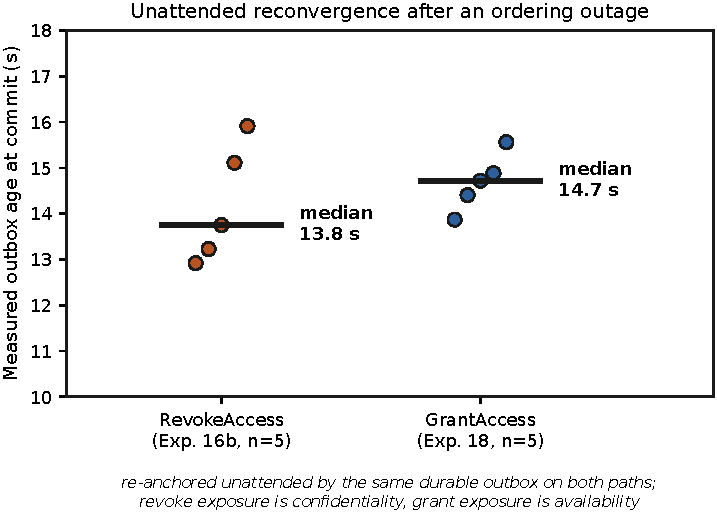
\includegraphics[width=\columnwidth]{fig18_write_divergence.pdf}
    \caption{Unattended reconvergence after an ordering outage, both
    access-control mutation paths. The two windows are statistically
    indistinguishable because the same durable outbox bounds both; the
    exposures they close are mirror images.}
    \label{fig:write_divergence}
\end{figure}

The bound generalizes beyond the near-zero outage measured here. Writing
$T_{\text{rec}}$ for the reconciliation lag, the retry schedule caps it at the
backoff ceiling plus Raft re-election and one commit, $T_{\text{rec}} \le c +
t_{\text{elect}} + t_{\text{commit}}$; for a near-zero outage the floor is
$t_{\text{elect}} + \delta + t_{\text{commit}}$ with $\delta$ the 5\,s poll. Both
measured medians sit inside that predicted floor band, and their agreement across
two different chaincode functions is itself evidence that the window is a
property of the reconciliation machinery rather than of either operation. The
saturated regime --- an outage long enough to drive the schedule to its cap ---
is still not exercised, and remains the one untested corner of the curve.

The remaining availability-first write is document registration, and it is left
that way deliberately: an unanchored registration denies the owner rather than
over-serving anyone, since the release path never authorizes from a registration
the ledger has not committed. Its divergence is in the safe direction, so it
carries no outbox.


\subsection{Scalability and standing costs}

Three questions about what the deployment costs to keep running rather than to
use: how cost grows with the archive, with the consortium, and with time. The
third exists only because of the mechanism that makes grant expiry trustworthy,
and it is the one that is easy to miss. Fig.~\ref{fig:ledgergrowth} plots both
of the growth terms together.

\subsubsection{Scale in documents}
\label{sec:exp_ledgergrowth}

Query cost is flat and storage is linear (Table~\ref{tab:docscale}). The
archive was loaded by 200 closed-loop submitters over 3.6 hours with zero
failures and sampled at each decade; the final point lands within 0.1\,\% of
the extrapolation from the previous decade, and the latency absolutes belong
to the build measured; the flatness is the transferable result. Across a
thousandfold increase in world state the access decision rises 0.64\,ms, about
8\,\%, and history retrieval 1.44\,ms at constant depth: the state lookup does
not degrade with archive size, which is the property that matters when the check
sits on every download. Storage runs at roughly \textbf{7\,KB per document per
peer} (5.6\,KB of block store plus 1.4\,KB of state database), so a million
documents occupy about 7\,GB per peer. Re-measuring the constant after the
authorization changes found 5{,}751\,B per document against the earlier
5{,}618, within noise; the premise that requiring an explicit grant for every
principal would enlarge each document's access map was simply wrong, because
registration has always written an explicit owner grant.

\begin{table}[!t]
\centering
\caption{Scale in document volume: per-peer storage and read latency at each
decade of world state.}
\label{tab:docscale}
\footnotesize
\setlength{\tabcolsep}{5pt}
\begin{tabular}{@{}rrrrr@{}}
\toprule
Documents & Block store & State DB & \texttt{CheckAccess} & History \\
\midrule
$10^3$ & 5.8\,MB     & 2.0\,MB     & 7.96\,ms & 5.68\,ms \\
$10^4$ & 56.5\,MB    & 14.0\,MB    & 7.07\,ms & 5.82\,ms \\
$10^5$ & 561.5\,MB   & 135.8\,MB   & 7.58\,ms & 6.01\,ms \\
$10^6$ & 5{,}618\,MB & 1{,}390\,MB & 8.60\,ms & 7.12\,ms \\
\bottomrule
\end{tabular}
\end{table}

Three limits belong with these numbers. \emph{No idle growth rate is reported
for the state database}: it compacts, so the series is a sawtooth and a fitted
slope is not a growth rate: a naive fit returns \emph{negative} 13\,MB per
day at $R^2 = 0.043$, and the analysis script detects the non-monotonicity and
refuses to emit a rate rather than printing it. Only the append-only block store
yields a durable rate. \emph{The re-measured state-database figure is an upper
bound}, taken from a burst containing no compaction. And \emph{the
million-document point was not re-validated on the current build}: the
re-measurement registered two thousand documents and re-checks the per-document
constant only. The original campaign established linearity across three orders
of magnitude and nothing here challenges it, but only the constant has been
re-checked.

\subsubsection{Scale across consortium size}
\label{sec:exp_netscale}

Consortium size is not what limits the write path (Table~\ref{tab:netscale}).
Across complete networks at
two, three, five and seven organizations, write throughput declines
\textbf{5.5\,\%} under single-organization endorsement, with write latency
pinned near the batch window throughout, the same ordering ceiling as
Section~\ref{sec:exp_throughput}. The majority-endorsement premium grows
sub-linearly, from 0.9\,\% at two organizations to 1.6\,\% at three, 5.4\,\% at
five and 12.7\,\% at seven, because the gateway collects endorsements in
parallel and the cost tracks the slowest endorser rather than their sum. That is
the quantity a deployment actually chooses when it sets its policy, and at
realistic sizes it is a single-digit percentage. Doubling peers within an
organization costs 3.3\,\%, against 5.5\,\% for growing the consortium from
two organizations to seven,
so replication for availability is cheap relative to admitting a member. Across
all nine points and both policies the access decision showed no trend in
organization count, which is what the mechanism predicts: it is a keyed state
lookup that never consults channel membership.

\begin{table}[!t]
\centering
\caption{Consortium size against write throughput and read latency, both
endorsement policies, 18{,}000 writes with zero failures.}
\label{tab:netscale}
\footnotesize
\setlength{\tabcolsep}{5pt}
\begin{tabular}{@{}rlrrr@{}}
\toprule
Orgs & Policy & Write TPS & Write P50 & Read P50 \\
\midrule
2 & single   & 43.3 & 2{,}297\,ms & 5.15\,ms \\
2 & majority & 42.9 & 2{,}322\,ms & 4.69\,ms \\
3 & single   & 42.8 & 2{,}325\,ms & 3.93\,ms \\
3 & majority & 42.1 & 2{,}363\,ms & 5.44\,ms \\
5 & single   & 42.3 & 2{,}358\,ms & 5.12\,ms \\
5 & majority & 40.0 & 2{,}482\,ms & 4.78\,ms \\
7 & single   & 40.9 & 2{,}432\,ms & 4.63\,ms \\
7 & majority & 35.7 & 2{,}785\,ms & 5.46\,ms \\
\bottomrule
\end{tabular}
\end{table}

All nine topologies ran in one campaign on one host, so the ratios between
rows are internally paired.
The matrix was not re-measured after the read-path changes, deliberately:
rebuilding networks up to seven organizations on a memory-constrained host is
exactly where this host has already failed once, and repeating the campaign
under worse conditions would most likely produce results
Section~\ref{sec:testbed}'s quiescence requirement obliges us to discard.
Absolute read latencies here are therefore stale, and
Section~\ref{sec:exp_latency} is the authority for the current build. What
transfers is the \emph{shape} (no dependence on consortium size), which is
what the experiment measured and what the mechanism explains. That the same
independence holds at the new level is a reasonable inference from the
mechanism; it is not a measurement, and we report it at that strength.

A consortium's firms are not in one building, so the reference
three-organization deployment was re-measured under injected round-trip delay. With delay on the client path only, throughput falls
\textbf{11\,\%} from 0 to 150\,ms RTT (68.2 to 60.8\,TPS, write P50 2{,}140 to
2{,}457\,ms). Delaying inter-orderer Raft traffic as well costs
\textbf{44.8\,\%} (69.5 to 38.3\,TPS, write P50 3{,}588\,ms); the cost is consensus
round trips, not the authorization decision, and it is the reason a geographically
split ordering service is the expensive choice. Both configurations remain
inside RQ2's five-second write budget at every point measured.

\subsubsection{Clock trust and its cost}
\label{sec:exp_timeanchor}

Grant expiry is evaluated inside \texttt{CheckAccess} against the transaction
timestamp. On an \emph{evaluate} that value originates in the calling client's
proposal, and under custodial submission the calling client is the application
gateway, precisely the component this architecture claims to remove from the
authorization trust boundary. So the relocation is weaker for expiry than for
membership: whether a grant \emph{exists} is read from committed state and
cannot be forged, but whether it has \emph{lapsed} is decided against a clock
the gateway supplies. A compromised gateway forges nothing; it constructs a
proposal carrying a timestamp from before the expiry instant, and signature
checking and endorsement do not detect it because nothing is forged. Per-user
enrollment would not help, since an evaluate is never ordered.

The mechanism that bounds this is a periodic time anchor committed by a
heartbeat submit. Because it is a submit, each endorsing peer independently
validates the heartbeat's timestamp against its own clock before endorsing, so a
backdated anchor cannot be committed without a colluding endorsement quorum,
itself already an assumption of the threat model. \texttt{CheckAccess} then refuses any
proposal more than a fixed tolerance behind the committed anchor. The gateway
cannot rewind the anchor; it can only starve it, and capping that is the job of
the staleness ceiling.

\paragraph{Latency cost of the freshness read}
The mechanism adds one world-state read to every access decision. On the
generation then deployed that read cost \textbf{+0.78\,ms} at the median (7.25
against 8.04\,ms, $n=150$ per arm, $p<10^{-15}$). That figure does not describe
the shipped build: repeating the identical paired toggle on the current
chaincode generation ($n=200$ per arm) found a mean difference of $-0.10$\,ms,
90\,\% confidence interval $[-0.63, +0.42]$\,ms, $p = 0.75$, and the earlier
value lies outside that interval. The two are not strictly contradictory
(different chaincode generations, world state and host sessions), but they
cannot both be quoted as the current price. \textbf{On the shipped build the
freshness read's cost is not detectable, and is bounded above by roughly
0.6\,ms at 90\,\% confidence.} A plausible mechanism is that the anchor key is
now hot, since the heartbeat rewrites it every 60\,s and every decision reads
it; that is an unmeasured hypothesis and we do not report it as a finding.

\paragraph{The security--availability trade-off}
The staleness ceiling is both halves of the trade at once: it is the
availability window (how long ordering can be unavailable before valid
decisions start being refused), and it sets the backdating bound. Two
constants compose that bound. The decision refuses any proposal whose
timestamp sits more than a fixed skew tolerance (120\,s as deployed)
behind the committed anchor, and refuses outright once the anchor itself is
more than the ceiling stale; a gateway that suppresses heartbeats can
therefore backdate by at most the ceiling plus the skew tolerance, which is
the bound tabulated. Sweeping the ceiling with the heartbeat stopped and the
release path polled every three seconds (Table~\ref{tab:staleness}), each
measured window tracks its configured value to within the poll granularity. Every second
of backdating tolerance bought is a second of outage tolerance surrendered, so
the curve is a straight line of unit slope and \emph{no setting improves both}.
With the ceiling disabled the release path kept authorizing for the full 200\,s
observation window with the anchor frozen. Zero is the shipped default,
the weaker security posture chosen for availability. Choosing otherwise is a
deployment judgment about which failure is less acceptable rather than a strict
improvement, the same trade as write-side divergence
(Section~\ref{sec:exp_divergence}) and deliberately priced once here for both.

\begin{table}[!t]
\centering
\caption{Staleness ceiling against the measured availability window; the
backdating bound is the ceiling plus the fixed 120\,s skew tolerance.}
\label{tab:staleness}
\footnotesize
\setlength{\tabcolsep}{6pt}
\begin{tabular}{@{}lrrl@{}}
\toprule
Ceiling & Availability window & Backdating bound & Outcome \\
\midrule
30\,s  & 31\,s  & 151\,s & refused \\
60\,s  & 59\,s  & 179\,s & refused \\
120\,s & 121\,s & 241\,s & refused \\
0 (disabled, shipped) & none within 200\,s & unbounded here & still authorizing \\
\bottomrule
\end{tabular}
\end{table}

\paragraph{Idle storage growth}
Because the heartbeat is a submit it writes a block whether or not anything else
occurs. With \textbf{zero} document activity the block store grew at a constant
\textbf{7.84\,MB per day per peer}: 90.7 bytes per second at $R^2 = 1.0000$ over
a twenty-minute idle window, exactly 1.00 blocks per minute against one
heartbeat per minute, so the attribution is exact rather than inferred. That is
$\sim$2.86\,GB per peer per year and $\sim$28.6\,GB over a decade: roughly
\emph{four times} what a million documents occupy, for an archive that never
receives another document. So the model is not linear in documents. It is
\begin{equation}
  S = a \cdot \mathit{documents} + b \cdot \mathit{time},
  \label{eq:storage_model}
\end{equation}
and the earlier campaign never measured $b$ because $b$ did not exist when it
ran. This remains commodity-hardware territory, which is the paper's actual
claim, but ``storage grows linearly with document count'' is no longer a
complete description of the cost, and we do not state it. The time term is a
price rather than a defect, and it is tunable: a five-minute interval costs a
fifth as much storage, traded against a proportionally looser backdating bound.
The heartbeat interval is the single parameter setting both.

\paragraph{Evidential standing of these claims}
Three propositions here have markedly different evidential standing, and we
separate them rather than let the presence of tests imply uniform support.
\emph{Measured:} the latency cost of the freshness read, the enforcement of the
staleness ceiling, and the standing storage cost. \emph{Unit-tested only,
against a mock stub:} that the release path refuses a proposal far behind the
anchor, that the anchor refuses to move backward, and that a live grant is still
authorized under a stale anchor. \emph{Argued, not tested:} that a compromised
gateway cannot commit a backdated \emph{anchor}: this rests on each endorsing
peer validating the heartbeat timestamp against its own clock, and multi-peer
endorsement is exactly what a single mock stub cannot exercise.

The third is the load-bearing claim and the least evidenced. No backdated
proposal was ever constructed against the
deployment: neither the peer command-line client nor the gateway SDK exposes the
proposal timestamp, so demonstrating the attack requires hand-building and
signing the proposal structure, and it was not attempted. The sweep's anchor
goes stale because heartbeats stop, which reconstructs the condition a
suppressing gateway would create without demonstrating the attack itself.

\begin{figure}[!t]
    \centering
    
\includegraphics[width=\columnwidth]{fig12_ledger_growth.pdf}
    \caption{Ledger growth along both scale axes, documents and time; total
    cost follows Eq.~\ref{eq:storage_model}.}
    \label{fig:ledgergrowth}
\end{figure}


\subsection{Comparison against a durable audit-log baseline}
\label{sec:exp_durable_baseline}

Section~\ref{sec:exp_latency} prices the authorization decision in isolation;
this experiment prices the whole architecture against the design it is proposed
to replace. The comparison turns entirely on how well the baseline is built, and
getting that right reversed the result.

An audit-log-only baseline built the obvious way measures \emph{faster} than
on-path enforcement, but the comparison is unfair in its favor. Its anchoring is
fire-and-forget through an in-memory queue: anchors drain at 3--8 per second
against hundreds generated, and the backlog was discarded when the process
stopped. A baseline whose audit trail evaporates on restart is not the
audit-log-only architecture but a naive implementation of it. The rebuilt
pipeline commits audit rows to the operational store before any anchoring is
attempted, so the backlog is on disk by construction; anchoring is batched, with
each batch hashing a contiguous range of audit-log identifiers and a watermark
marking the highest committed range, because the audit log is append-only and
enforced by a trigger that would make per-row bookkeeping impossible without
relaxing the tamper evidence the design rests on. Against a genuine 39{,}450-row
backlog it drained at \textbf{53.3 events per second}, roughly ten times the
naive rate.

\begin{table}[!t]
\centering
\caption{Release-path throughput and latency for three architectures under
an identical read-only download workload, 1{,}000 requests per level, zero
failures in every cell.}
\label{tab:durable_baseline}
\footnotesize
\setlength{\tabcolsep}{5pt}
\begin{tabular}{@{}lrrrr@{}}
\toprule
& \multicolumn{2}{c}{concurrency 10} & \multicolumn{2}{c}{concurrency 50} \\
\cmidrule(lr){2-3}\cmidrule(lr){4-5}
Mode & TPS & P50 & TPS & P50 \\
\midrule
A. On-path enforcement                 & \textbf{469.5} & \textbf{16.6\,ms} & \textbf{789.6} & \textbf{59.2\,ms} \\
B. Audit-log-only, fire-and-forget     & 393.4 & 15.6\,ms & 557.9 & 57.3\,ms \\
C. Audit-log-only, durable batched     & 142.3 & 32.8\,ms & 226.9 & 209.3\,ms \\
\bottomrule
\end{tabular}
\end{table}

Table~\ref{tab:durable_baseline} and Fig.~\ref{fig:durable_baseline} invert the
earlier finding. Against the naive
mode~B, on-path enforcement costs essentially nothing at the median and is
faster in throughput; against mode~C, the baseline that keeps its promise, it
delivers \textbf{3.3$\times$ the throughput and half the median latency} at
concurrency~10 and 3.5$\times$ at concurrency~50. Durability behaved as
designed: mode~B left 69 anchors unrecoverable in memory once the process
exited, while mode~C left 16 in flight on disk across 318 committed batches with
the watermark still advancing.

The gap is structural rather than a tuning artifact. In the audit-log-only
architecture the anchor \emph{is} the security mechanism (if it never reaches
the ledger there is no ledger-verifiable record of the decision), so the
pipeline must be durable and must sustain the request rate. In the on-path
design the decision is taken before release, so the anchor is telemetry and need
be neither. One architecture pays for durability on every decision; the other
does not have to. Making the baseline fair therefore does not rescue it: it
makes it slower, because the cost the naive implementation avoids is one that
architecture has to pay.

\paragraph{Equivalence against the naive baseline, tested as such}
One sign here runs opposite to Section~\ref{sec:exp_latency}, and the two
measure different things. That section isolates the authorization decision, where
a chaincode evaluate costs 4.0 to 4.4\,ms more than a local database query and
nothing else differs between arms. This one prices whole architectures, in which
the database-deciding arm also carries asynchronous anchoring work that on-path
enforcement does not. A cheaper decision inside a more expensive architecture is
not a contradiction. The end-to-end difference between modes A and B at
concurrency~10 is $-4.08$\,ms, with a 90\,\% confidence interval of
$[-5.63, -2.52]$\,ms lying entirely inside RQ2's pre-specified $\pm 50$\,ms
margin; two one-sided tests give $p < 10^{-15}$. The direction is visible in the
dispersion, the database-deciding arm carrying roughly double the standard
deviation because its anchoring work lands unevenly on the request path.

Three caveats bound this. \emph{The sweep is reduced}, to two concurrency levels
and half the requests per level of the original campaign, so the saturation
behavior previously reported at concurrency 100 and 200 is not re-validated and
no claim about it is carried forward. \emph{Mode~A's own audit events are
deliberately not durably anchored}: that is the asymmetry being argued rather
than an oversight, since each mode is built as it must be to keep its own
promise. And \emph{the A-versus-B direction
disagrees with our earlier run}, in which the baseline was faster; the system has
since gained the freshness read, lost the organization fallback and begun
anchoring denials, so the two campaigns' absolutes must not be mixed. One probe of the same question ran under an instrument defect and is listed
with the other exclusions in Table~\ref{tab:excluded}.

\begin{figure}[!t]
    \centering
    
\includegraphics[width=\columnwidth]{fig14b_durable_baseline.pdf}
    \caption{On-path enforcement against both audit-log-only baselines:
    (a) throughput, (b) latency, at the two measured concurrency levels.}
    \label{fig:durable_baseline}
\end{figure}


\subsection{Consolidated evidence}
\label{sec:exp_consolidated}

Table~\ref{tab:consolidated} gathers the headline measurements with their
intervals, including several this paper does not otherwise give a section to.
It exists for two reasons: to let a reader check any figure quoted elsewhere
against its interval and its source, and to make visible how much of the
campaign rests on single runs rather than replicates.

It follows Section~\ref{sec:testbed}'s conventions throughout, and is generated
from the released per-sample data by a script with a fixed resampling seed, so
it is reproducible rather than transcribed. Rows without an interval are
categorical outcomes or single-run measurements, marked rather than given
a spurious one, a distinction worth attending to, because three of the results
this paper leans on are counts rather than distributions.

\begin{table}[!t]
\centering
\caption{Consolidated evidence with 95\,\% confidence intervals, generated
from the released data at a fixed seed.}
\label{tab:consolidated}
\scriptsize
\setlength{\tabcolsep}{3pt}
\begin{tabular}{@{}>{\raggedright\arraybackslash}p{0.42\columnwidth}rrl@{}}
\toprule
Metric & $n$ & Value & 95\,\% CI \\
\midrule
\multicolumn{4}{@{}l}{\emph{Read-path cost} (Section~\ref{sec:exp_latency})}\\
\quad \texttt{CheckAccess} P50, ledger, pooled brackets & 200 & 10.99\,ms & [10.71, 11.25] \\
\quad \texttt{CheckAccess} P50, database lookup          & 100 & 6.44\,ms  & [6.21, 6.70] \\
\quad \texttt{RegisterDocument} P50                      & 100 & 2087\,ms  & [2086.4, 2088.2] \\
\midrule
\multicolumn{4}{@{}l}{\emph{Capacity} (Section~\ref{sec:exp_throughput})}\\
\quad Gateway throughput, default batch window  & 5  & 66.3\,TPS & [63.7, 68.9] \\
\quad Gateway throughput, 500\,ms batch window  & 10 & 193.0\,TPS & [182.8, 203.2] \\
\midrule
\multicolumn{4}{@{}l}{\emph{Failure behavior} (Sections~\ref{sec:exp_failclosed}, \ref{sec:exp_divergence})}\\
\quad Protected bytes released during outage & --- & 0 & categorical \\
\quad Fail-closed denials during the outage  & --- & 1{,}340 & categorical \\
\quad Revocation divergence window to convergence & 5 & 15.92\,s & [14.86, 16.51] \\
\quad Grant divergence window to convergence      & 6 & 14.35\,s & [13.01, 15.78] \\
\midrule
\multicolumn{4}{@{}l}{\emph{Adversarial} (Sections~\ref{sec:exp_db_mutation}, \ref{sec:exp_pubkey})}\\
\quad Ciphertext released on a forged database grant & --- & 0 & categorical \\
\quad Wrapped keys released on a forged grant        & --- & 0 & categorical \\
\quad Key material released on a substituted public key & --- & 0 & categorical \\
\midrule
\multicolumn{4}{@{}l}{\emph{Scale} (Sections~\ref{sec:exp_ledgergrowth}, \ref{sec:exp_netscale})}\\
\quad \texttt{CheckAccess} P50 at $10^3$ documents & 100 & 7.96\,ms & --- \\
\quad \texttt{CheckAccess} P50 at $10^6$ documents & 100 & 8.60\,ms & --- \\
\quad Block store per document                     & 2{,}000 & 5{,}751\,B & rate \\
\quad Idle growth, zero document activity          & 21 & 7.84\,MB/day & rate \\
\midrule
\multicolumn{4}{@{}l}{\emph{Architectural comparison} (Section~\ref{sec:exp_durable_baseline})}\\
\quad Release P50, on-path enforcement            & 1{,}000 & 16.55\,ms & [16.20, 16.95] \\
\quad Release P50, audit-log-only, durable        & 1{,}000 & 32.75\,ms & [31.30, 34.30] \\
\midrule
\multicolumn{4}{@{}l}{\emph{Compressed experiments}, reported only here}\\
\quad Fabric commit latency, size-independent      & 10 & 2{,}132\,ms & size-invariant \\
\quad Audit query P50, operational store           & 10 & 3.90\,ms & \\
\quad History retrieval P50 at depth 107           & 10 & 135.5\,ms & \\
\quad Storage retrieval P50, 50\,MB, cross-node    & 10 & 875\,ms & \\
\quad Throughput at 150\,ms RTT, Raft delayed      & 5 & $-44.8$\,\% & per point \\
\bottomrule
\end{tabular}
\end{table}

\subsubsection*{What the consolidation shows that individual sections do not}

Three observations only become visible once the measurements sit together.

\emph{The ledger decision is stable across independent setups.} It lands
between roughly 8 and 11\,ms in four separate configurations (the
function-level comparison, both ends of the document-volume sweep, and across
consortium sizes), despite those runs spanning months, different world-state
sizes, and different builds. The absolutes are not comparable across those
builds, and we do not treat their agreement as a measurement. It is
nonetheless the kind of coherence whose absence would be a warning.

\emph{Several results are counts, not distributions.} Zero protected bytes
released, zero forged-grant releases, 1{,}340 denials: these carry no interval
because there is no sampling distribution to describe, and no amount of
resampling would make them stronger. What makes them credible is that the
quantity being counted is a violation, and the count is zero.

\emph{The compressed rows are not weak results, but they are thin.} File-size
independence, audit-query cost, history depth and storage retrieval each rest on
ten samples of a single configuration; the RTT sweep is five trials at each of
eight points. They are reported here rather than in
sections of their own because each supports a claim no part of this paper
depends on, and giving them equal weight would misrepresent where the evidence
is concentrated.

\subsubsection*{Comparison with reported figures from other systems}

We report no head-to-head benchmark against the systems in
Section~\ref{sec:related}, and would caution against constructing one from
published numbers. The closest system reports contract execution in
1--2\,ms against our 10.99\,ms, but the two measure different things on
different hardware: theirs is contract execution time on a storage-layer hook,
ours is an end-to-end decision through an application gateway including the
network round trip. Neither number is wrong and neither bounds the other. The
comparison that does transfer is architectural, not numerical, and it is
Table~\ref{tab:related}.


\section{Discussion}
\label{sec:discussion}

\subsection{Access-graph disclosure}
\label{sec:accessgraph}

Making an authorization decision independently verifiable requires that
consortium members can see the state it was evaluated against. That state is an
access graph: who was granted what, by whom, when, and until when. In
litigation the graph is not incidental metadata. It is frequently more
sensitive than the documents.

Four disclosures follow directly, and none requires decrypting anything.
\emph{Expert retention} becomes visible: granting access to an outside expert
reveals that the expert was retained, and when, which a party may be entitled
to withhold until a disclosure deadline. \emph{Review-team composition}
becomes visible, and with it staffing levels and, by inference, how a matter is
being resourced. \emph{Production scope} becomes visible: the set of documents
granted to opposing counsel is a statement about what the producing party
considers responsive, and the shape of that set can be read strategically. And
\emph{ethical walls invert}: the mechanism that would let a party prove a wall
was respected is the same mechanism that reveals precisely who is walled off
from what.

The obvious mitigation is to move grant state into a private collection, so
that only its members see the graph while the wider channel sees a commitment
to it. This is not a pure improvement. The verification property that motivates the whole architecture is that a party
outside the deciding organization can check an access decision against
committed state. Narrowing who holds that state narrows who can perform that
check. A regulator or court-appointed reviewer outside the collection would
lose exactly the capability the design exists to provide, and the endorsement
requirements of the decision itself change with it.

So this is a design tension rather than a defect with a fix. A deployment must
decide whose verification matters more: the counterparty's, which argues for
broad visibility, or the producing party's confidentiality in its own
litigation posture, which argues for narrow. It is not resolved here.

A related question arises for retention. The architecture keeps document
content off-chain and erasable (unpinning and collecting a stored object
removes it), while the ledger retains hashes, identifiers, and timestamps
permanently. Whether those residues constitute personal data is
jurisdiction-dependent and contested~\cite{gdpr2016,lyons2018integration}, and
hash-based identifier replacement is analyzed as pseudonymization rather than
anonymization, leaving the result personal
data~\cite{Finck2020,EDPB2025Pseudonymisation}. The decomposition narrows the
problem; it does not dispose of it, and deployment under an erasure regime
needs a legal determination this paper does not supply.

\subsection{Clock trust as a standing cost}
\label{sec:clocktrustprice}

Making grant expiry trustworthy requires an ordered heartbeat
(Section~\ref{sec:exp_timeanchor}), and an ordered transaction writes a block
whether or not anyone uses the system. Paying for a security property in storage that accrues whether or
not anyone uses the system is an unusual shape of cost, and it hides from the
measurement that would normally catch it: it never appears under load, because
it does not scale with load (Section~\ref{sec:exp_ledgergrowth}). Two
independent parameters govern the trade: the heartbeat interval sets the
storage rate and the staleness ceiling sets the backdating bound. The
prototype ships with the ceiling disabled, preferring availability and accepting
the weaker bound. That is a deployment judgment about which failure is less
acceptable, and a legal deployment where expiry carries contractual weight may
reasonably choose differently.

\subsection{Threats to validity}
\label{sec:validity}

Limitations specific to individual measurements are stated where those
measurements are reported. Three cut across all of them.

Everything was measured on a single host running a three-organization
consortium. Absolute throughput is conservative as a result, and the
transferable quantities are ratios between arms measured in the same run rather
than absolute values, a constraint stated as method in
Section~\ref{sec:testbed} and observed throughout, most consequentially in
Section~\ref{sec:exp_netscale}, where the consortium-size result is reported as
ratios and its absolutes are scoped to the build that produced them.

The campaign spans several months and several system images, and the system
under test changed during it. Where a figure belongs to a superseded build we
say so rather than presenting it as current, and where two measurements of the
same quantity disagree, both are reported with the discrepancy explained.

Finally, the workload is synthetic. The steady-state rate against which
capacity is judged is a capacity-planning assumption about a
thousand-user firm, not a measurement of real legal traffic, and no part of
this paper validates it against production logs. The measured capacity
transfers; the margin over the baseline is only as good as the baseline.


\section{Conclusion and future work}
\label{sec:conclusion}

Placing an authorization decision on the document-release path is established
practice. What had not been reported is how such a design behaves when the
assumptions underneath it fail. This paper measured that, for a legal-document
consortium built on a permissioned ledger with encrypted off-chain storage, and
the answer is that the design fails asymmetrically.

Reads fail closed. Across an induced ledger outage no protected byte was
released, and the operational access-control list never authorized in the
ledger's place. An adversary holding write access to that list cannot obtain
protected material either: the forged grant is inert, because the ledger
decides. The decision costs 4.0 to 4.4\,ms more than a local database lookup:
a real difference rather than an equivalence, and a small one against the
threshold fixed before measuring.

Writes are availability-first and can diverge. An access-control change issued
while the ordering service is unavailable completes operationally without
reaching the ledger, and the two mutation paths fail in opposite directions: a
diverged revocation keeps authorizing a revoked user, a diverged grant keeps
refusing an authorized one. A durable outbox bounds both, reconverging unattended
in a median of 14 to 16\,s with intent order preserved. The asymmetry itself is
the contribution: which harm a diverged write produces is fixed by the
fail-closed read, so it follows from how reads and writes reach a ledger rather
than from anything particular to this implementation.

Two further results bear on whether the architecture is worth its cost. Against
an audit-log-only baseline rebuilt so that its audit trail survives a restart,
on-path enforcement sustains over three times the throughput. That reverses what
the same comparison showed against a careless baseline, and the reversal is
structural: in that architecture the anchor is the enforcement record, so it
must be durable. The second result is a standing cost that appears in no
throughput figure: the ordered heartbeat that makes grant expiry trustworthy
accrues 7.84\,MB per day per peer at zero document activity. Over a decade of
retention that exceeds the storage of a million documents.

The evidence for each of these, including the runs excluded and the criterion
that excluded them, is released alongside the paper.

\subsection*{Future work}

Three items follow directly from what this paper leaves open, in the order we
would attempt them.

\emph{Demonstrate the backdating attack, or rule it out.} The defense against a
gateway supplying its own clock is measured for cost and for enforcement. But
the load-bearing claim, that a compromised gateway cannot commit a backdated
anchor, rests on multi-peer endorsement, and has been argued rather than
tested. Doing so needs a client that assembles and signs proposals directly,
which neither the standard tooling nor the gateway software development kit
exposes. This is the one adversarial claim in the paper still argued rather than
measured, and it is where we would spend effort first.

\emph{Characterize the divergence curve at its bound.} The measured
reconciliation windows, on both mutation paths, come from a near-zero outage and
are therefore almost entirely recovery lag. How the window behaves under a
partial ordering outage, a rolling restart, or an outage long enough to drive the
retry schedule to its cap is not measured, and it is the question a deployment
would actually ask.

\emph{Complete the key-binding migration and prove the wrap.} Public-key
substitution is now refused at grant time and the wrapping construction now
interposes a KDF (Sections~\ref{sec:exp_pubkey}, \ref{sec:crypto}), but the
binding guarantee is advisory until every user enrolled before anchoring has had
their key back-anchored, after which absent-binding grants can be rejected by
configuration. With the KDF in place a machine-checked chosen-ciphertext proof of
the grant and wrapping protocols is now tractable, and is the formal companion
this measurement-first paper does not itself supply.

Three further directions are worth naming. Per-user ledger enrollment with
hardware-backed key storage would close the custodial-attribution gap, though
not the clock-trust assumption that follows from queries never being ordered.
Formal verification of the grant and wrapping protocols would supply the proofs
this work does not offer. Migration to Byzantine-fault-tolerant ordering is a
configuration path rather than a redesign. Whether to narrow access-graph visibility through private
collections is not future work but a deployment decision, and
Section~\ref{sec:accessgraph} argues that it trades away part of the
verifiability the architecture exists to provide.


\section*{CRediT authorship contribution statement}
\textbf{Golam Bari Fardeen:} Conceptualization, Methodology, Software,
Investigation, Writing -- original draft.
\textbf{Namare Shakib Angkon:} Methodology, Software, Visualization,
Writing -- original draft, Writing -- review \& editing.
\textbf{Syed Zayan Anwar:} Software, Validation, Formal analysis,
Writing -- review \& editing.
\textbf{Md.\ Masum Mizi:} Software, Resources, Visualization.
\textbf{Shinthia Rahman:} Resources, Validation.
\textbf{Md.\ Motaharul Islam:} Supervision, Funding acquisition.

\section*{Declaration of competing interest}
The authors declare that they have no known competing financial interests
or personal relationships that could have appeared to influence the work
reported in this paper.

\section*{Acknowledgments}
This work was supported by the Institute for Advanced Research Publication
Grant of United International University, under Grant IAR 2025 Pub 093.

\section*{Data availability}
The raw measurement data for the experiments reported in
Section~\ref{sec:performance} (per-sample CSVs with per-run environment
records), the load generators, topology generators, and analysis and plotting
scripts that produce every figure and table in this paper, together with the
measured-versus-manuscript reconciliation log, are archived as a citable
replication package at
\url{https://doi.org/10.5281/zenodo.XXXXXXX} (Zenodo), with the
development history available at
\url{https://github.com/meteorboyF/BCRA_paper_prototype}
(directories \texttt{results/} and \texttt{experiments/}, branch
\texttt{prototype-fixes}; the post-campaign two-host validation dataset,
including the client-side trial logs and RTT records, is on branch
\texttt{linux-validation}).

\section*{Declaration of generative AI and AI-assisted technologies in the
manuscript preparation process}
During the preparation of this work the authors used Claude (Anthropic) in
order to assist with language editing, manuscript structuring and \LaTeX{}
formatting. After using this tool, the authors reviewed and edited the
content as needed and take full responsibility for the content of the
published article.

\begingroup
\emergencystretch=2em
\bibliographystyle{elsarticle-num}
\bibliography{references}
\endgroup

\end{document}
